\chapter{Systematic Uncertainties}
\label{chap:systematics}

The nominal simulated shape of the \Nb distribution is allowed to vary by the inclusion of systematic uncertainties.
Each uncertainty is incorporated in the fit with template \Nb histograms to account for the effects of the systematic variation and a nuisance parameter $\theta$ to control the variation amplitude.
The nuisance parameters are subject to Gaussian constraints, normalized so that $\theta=0$ corresponds to the nominal \Nb shape and $\theta=\pm1$ corresponds to $\pm1$ standard deviation (s.d.)\ variation of the systematic uncertainty.
These uncertainties affect only the \Nb shape for \ttbar, QCD, and W+jets backgrounds, because their normalizations are determined from data, while for the other (subleading) backgrounds the uncertainties affect both the \Nb shape and normalization.

\begin{section}{Gluon Splitting Rate}

The primary source of systematic uncertainty is on the modelling of the rate of gluon splitting (GS), as events with a gluon splitting to \bbbar provide an additional source of b quarks in events.
As this process may not be properly simulated, constraining the splitting rate in data is crucial for establishing a robust prediction of the \Nb distribution.
The dominant contribution of this effect is due to gluons that split specifically to b~quark pairs, so the phrase ``gluon splitting'' will hereafter refer exclusively to gluon splitting to \bbbar.
One way to select a data sample enriched in gluon splitting events is to use the \dRbb distribution, where \dRbb is defined as the $\Delta R$ between two b-tagged jets, as pairs of b-tagged jets resulting from the same gluon splitting tend to have smaller values of \dRbb than pairs resulting from hard scatter b-quarks or mis-tagged jets.
This can be seen in Figure~\ref{fig:dRbb_shapes}, which shows the \dRbb distribution in simulated QCD events with $\Nb = 2$ for three important categories.
Events that have a correlated pair of b-tagged jets originating from a gluon splitting (green, denoted GSbb) populate the low-\dRbb region, while events without gluon splitting (yellow, denoted noGS) or where the splitting yields one or fewer b-tagged jets (blue, denoted GSb) populate the low-and high-\dRbb regions roughly equally.

\begin{figure}[tbp!]
\begin{center}
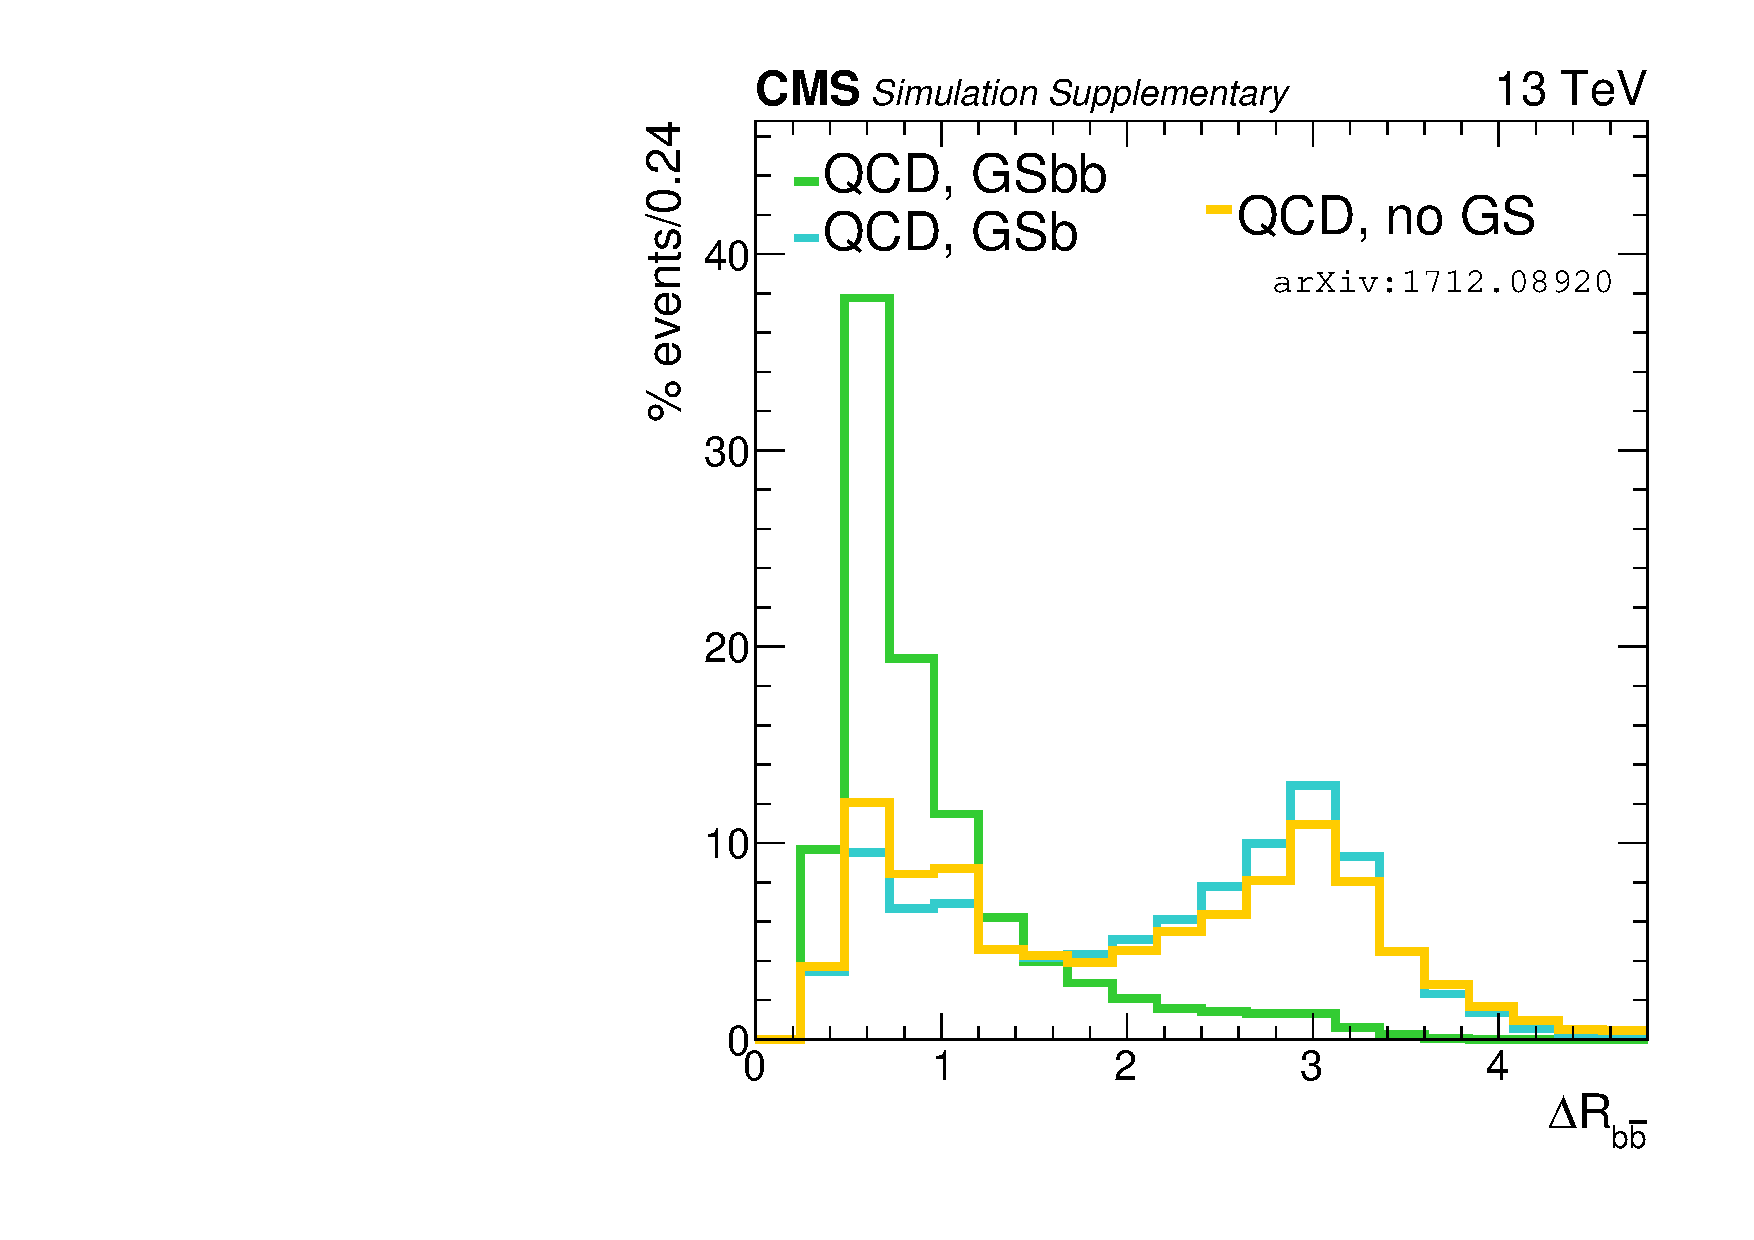
\includegraphics[angle=0,width=0.60\columnwidth]{fig/dRbb_shapes.pdf}
\end{center}
\caption{The \dRbb distribution shapes for the three gluon splitting categories: 
Events with a pair of b-tagged jets resulting from gluon splitting (green), events with a gluon splitting yielding fewer than 2 b-tagged jets (blue), and events without a gluon splitting to \bbbar.
These events are selected by requiring $\Nleps = 0$, $\HT > 1500~\GeV$, $\MJ > 500~\GeV$, $\Njets \geq 4$, and $\Nb = 2$.}
\label{fig:dRbb_shapes}
\end{figure}

Gluon splittings can contribute less than 2 b-tagged jets either because the quarks are collimated into a single jet, one of the b-tagged jets is not tagged, or because one of the jets fails to pass the jet selection criteria, typically because it is too soft.
The relative fractions of these contributions is shown in Figure~\ref{fig:gs_categories}.

\begin{figure}[tbp!]
\begin{center}
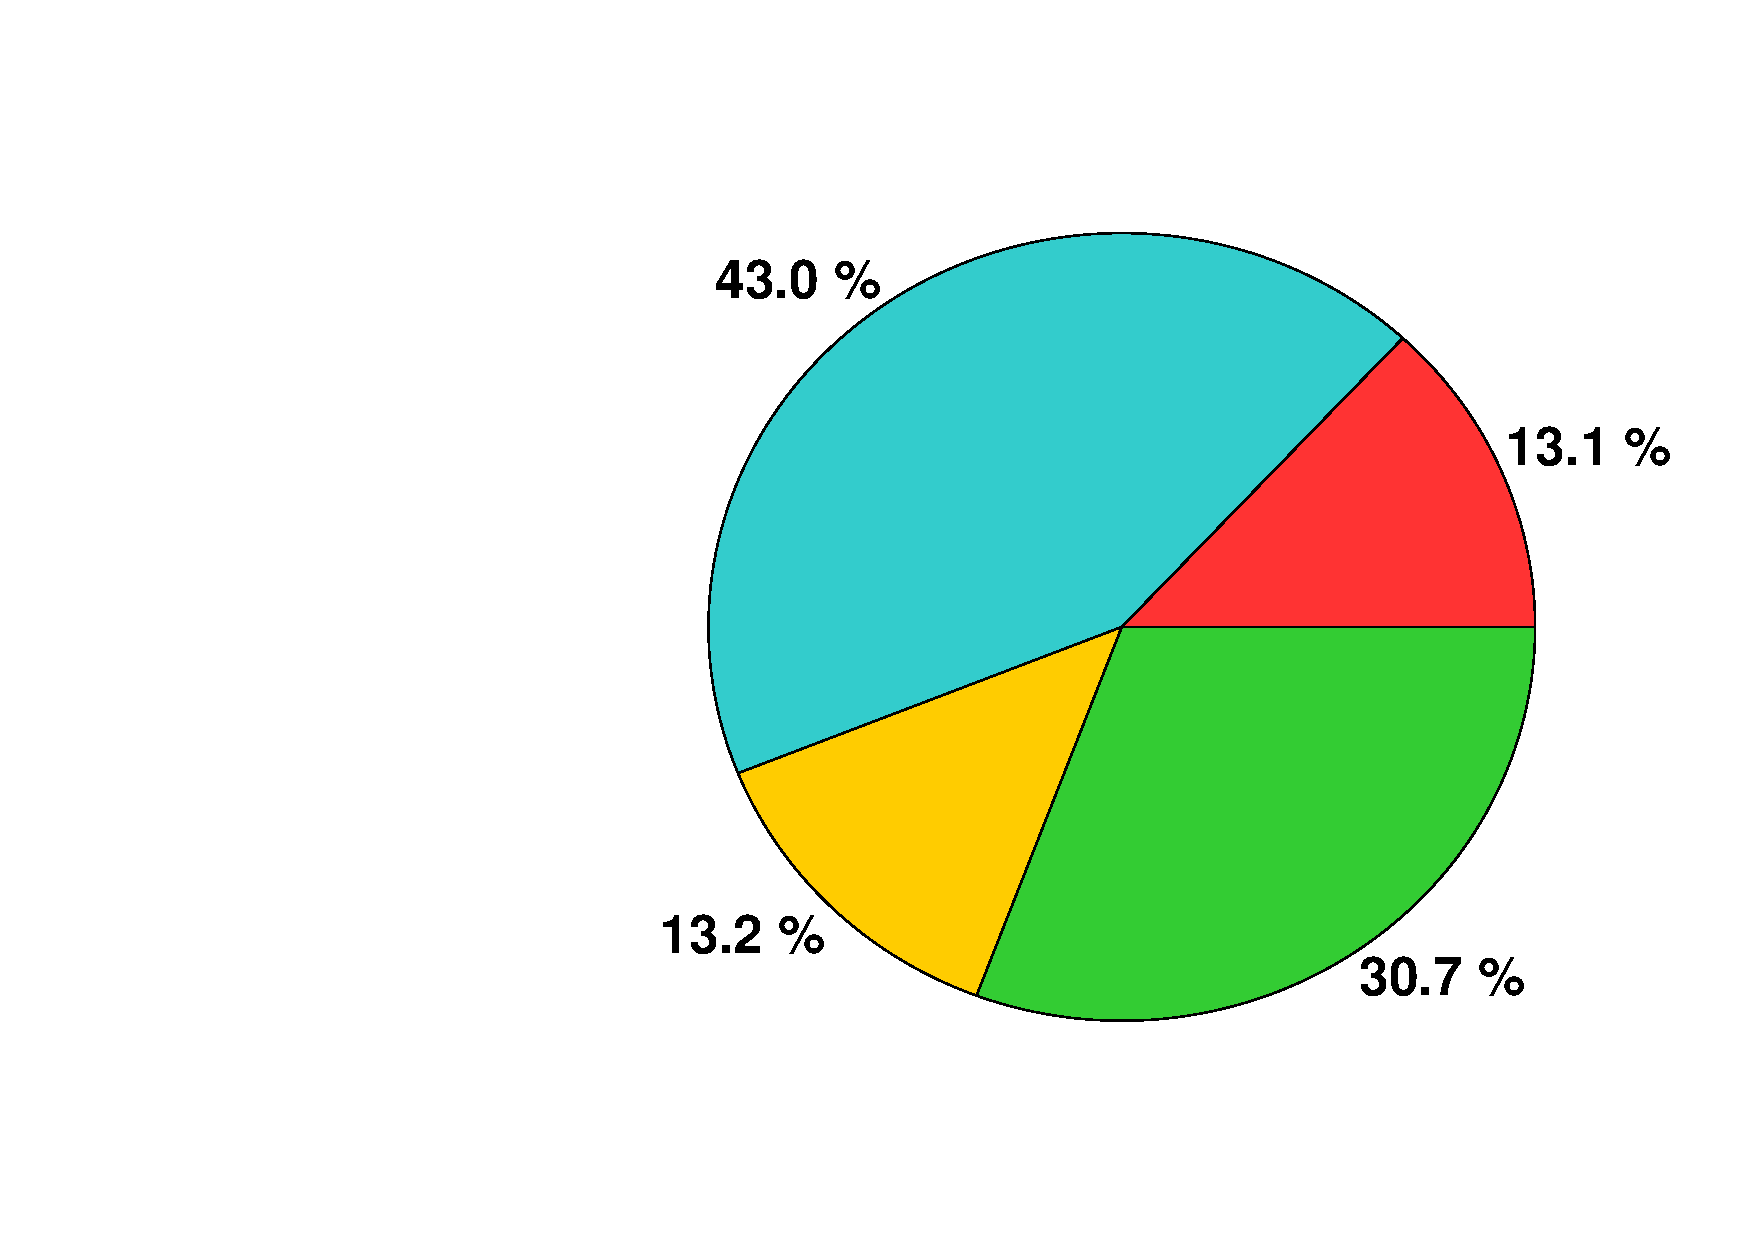
\includegraphics[angle=0,width=0.45\columnwidth]{fig/gs_piechart.pdf}
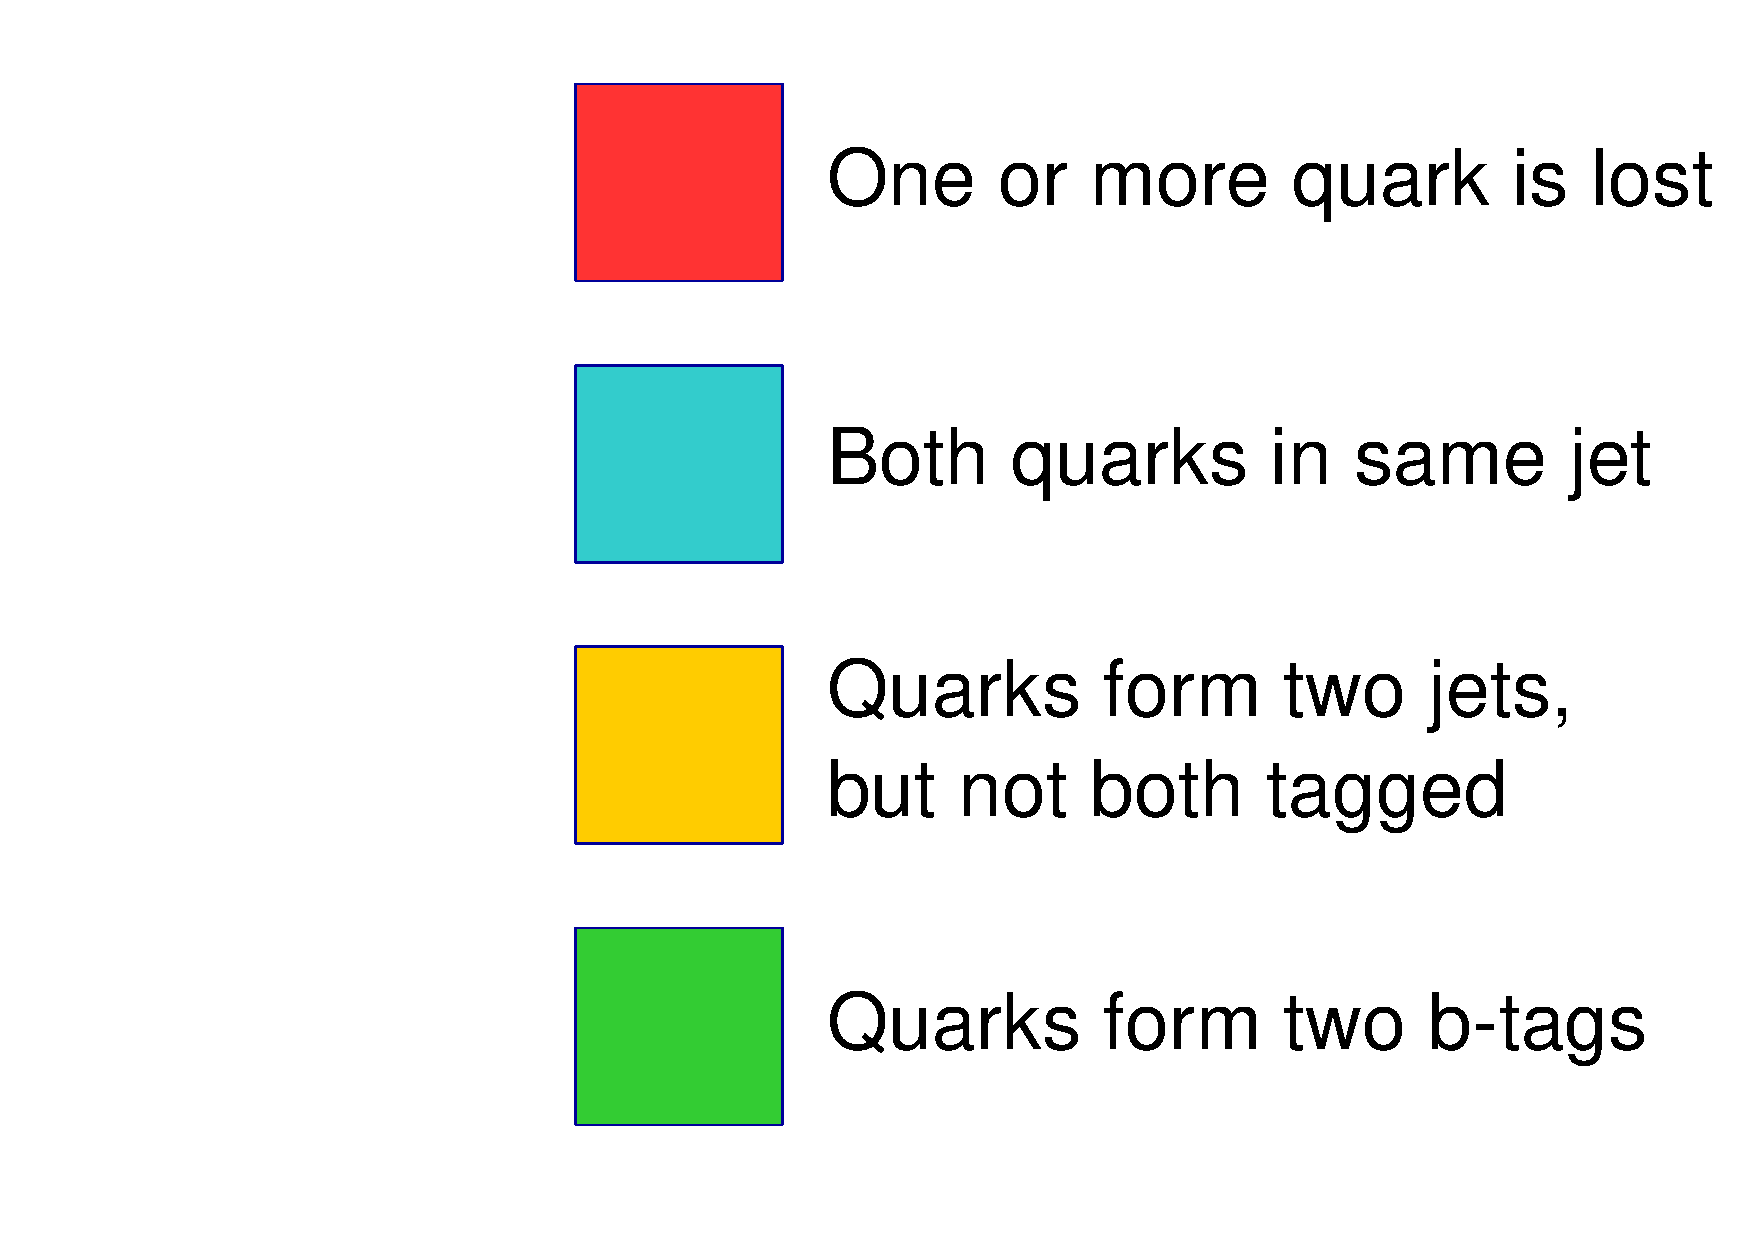
\includegraphics[angle=0,width=0.45\columnwidth]{fig/gs_piechart_legend.pdf}
\end{center}
\caption{The relative fraction of the possible final states that occur from gluon splitting to \bbbar for events satisfying $\Nleps = 0$, $\HT > 1500~\GeV$, $\MJ > 500~\GeV$, $\Njets \geq 4$, and $\Nb = 2$.}
\label{fig:gs_categories}
\end{figure}

The gluon splitting rate is then constrained by fitting the \dRbb distributions to data by using the difference in shapes of the GSbb, GSb, and noGS categories.
This fit varies the normalization of the GSbb and GSb contributions (varied together) and the noGS contributions in order to extract the relative contributions of events with and without a gluon splitting.
It is performed in four equal bins in the range of $0 \leq \dRbb < 4.8$ with events selected by requiring $\Nleps = 0$, $\HT > 1500~\GeV$, $\Nb = 2$, $\Njets \geq 4$, and $\MJ > 500~\GeV$, as the gluon splitting signal in a $\Nleps = 1$ control sample is contaminated by b~quarks from the decay of top quarks.
Additionally, the $\Nleps = 0$ control sample is formed from a subset of the data that is selected to be most stable in the b~tagging algorithm performance, since the precision of the \dRbb fit is not limited by the data sample size.
This choice isolates the physical effects of gluon splitting from the potential time dependence of the b~tagging performance due to variations in experimental conditions, which are separately incorporated by the uncertainties on the b-tagging data-to-simulation scale factors, as described in Section~\ref{sec:btag_sfs}.

The \dRbb fit extracts a weight of $0.77 \pm 0.09$ for gluon splitting events and a weight of $1.21 \pm 0.08$ for non-gluon splitting events.
The post-fit distributions are shown in Figure~\ref{fig:gs_fitresult}.
The GSbb and GSb categories are plotted separately to demonstrate the difference in shapes.
The discrepancy in the last bin does not significantly impact the fit because the higher yield bins at lower values of \dRbb constrain the fit.
The deviations of these weights from unity, summed in quadrature with their post-fit uncertainty, are used to form the $\pm 1$~s.d.\ variations of the gluon splitting rate nuisance parameter by applying weights of $1 \pm 0.25$ to gluon splitting events and $1 \mp 0.22$ to non-gluon splitting events in an anti-correlated manner.
The fit results are used as a measure of the uncertainty on modelling of the GS rate as opposed to a correction to the central value, since the \dRbb  variable may not be a perfect proxy for the GS rate.
Figure~\ref{fig:gs_variations} shows the effect of the $\pm 1$~s.d.\ variations on the \Nb distribution of \ttbar for the two most sensitive bins.

\begin{figure}[tbp!]
\begin{center}
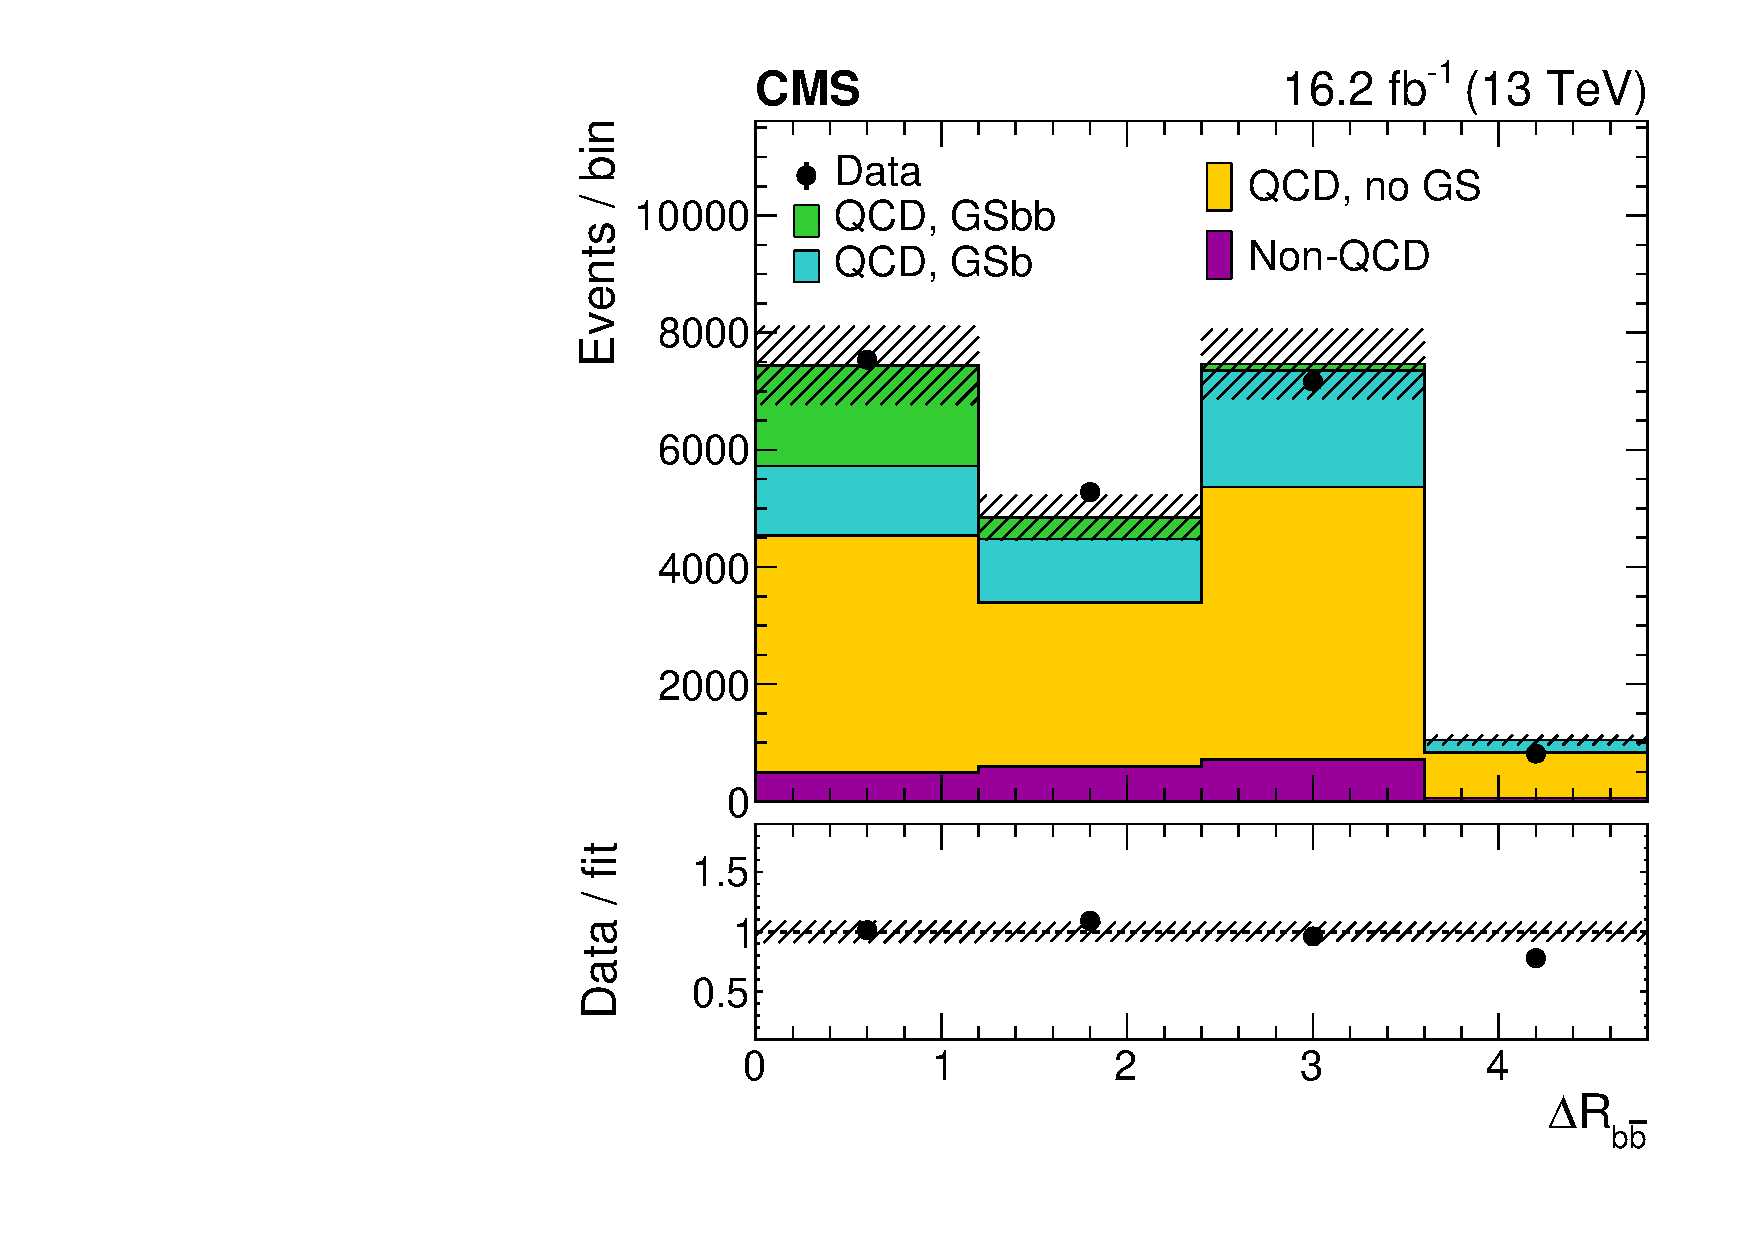
\includegraphics[angle=0,width=0.60\columnwidth]{fig/gs_fitresult.pdf}
\end{center}
\caption{Post-fit \dRbb distributions in a selection with  $\Nleps = 0$, $\HT > 1500~\GeV$, $\MJ > 500~\GeV$, $\Njets \geq 4$, and $\Nb = 2$ with the post-fit uncertainty represented by a hatched band.
The ratio of data to simulation yields is shown in the lower panel.}
\label{fig:gs_fitresult}
\end{figure}

\begin{figure}[tbp!]
\begin{center}
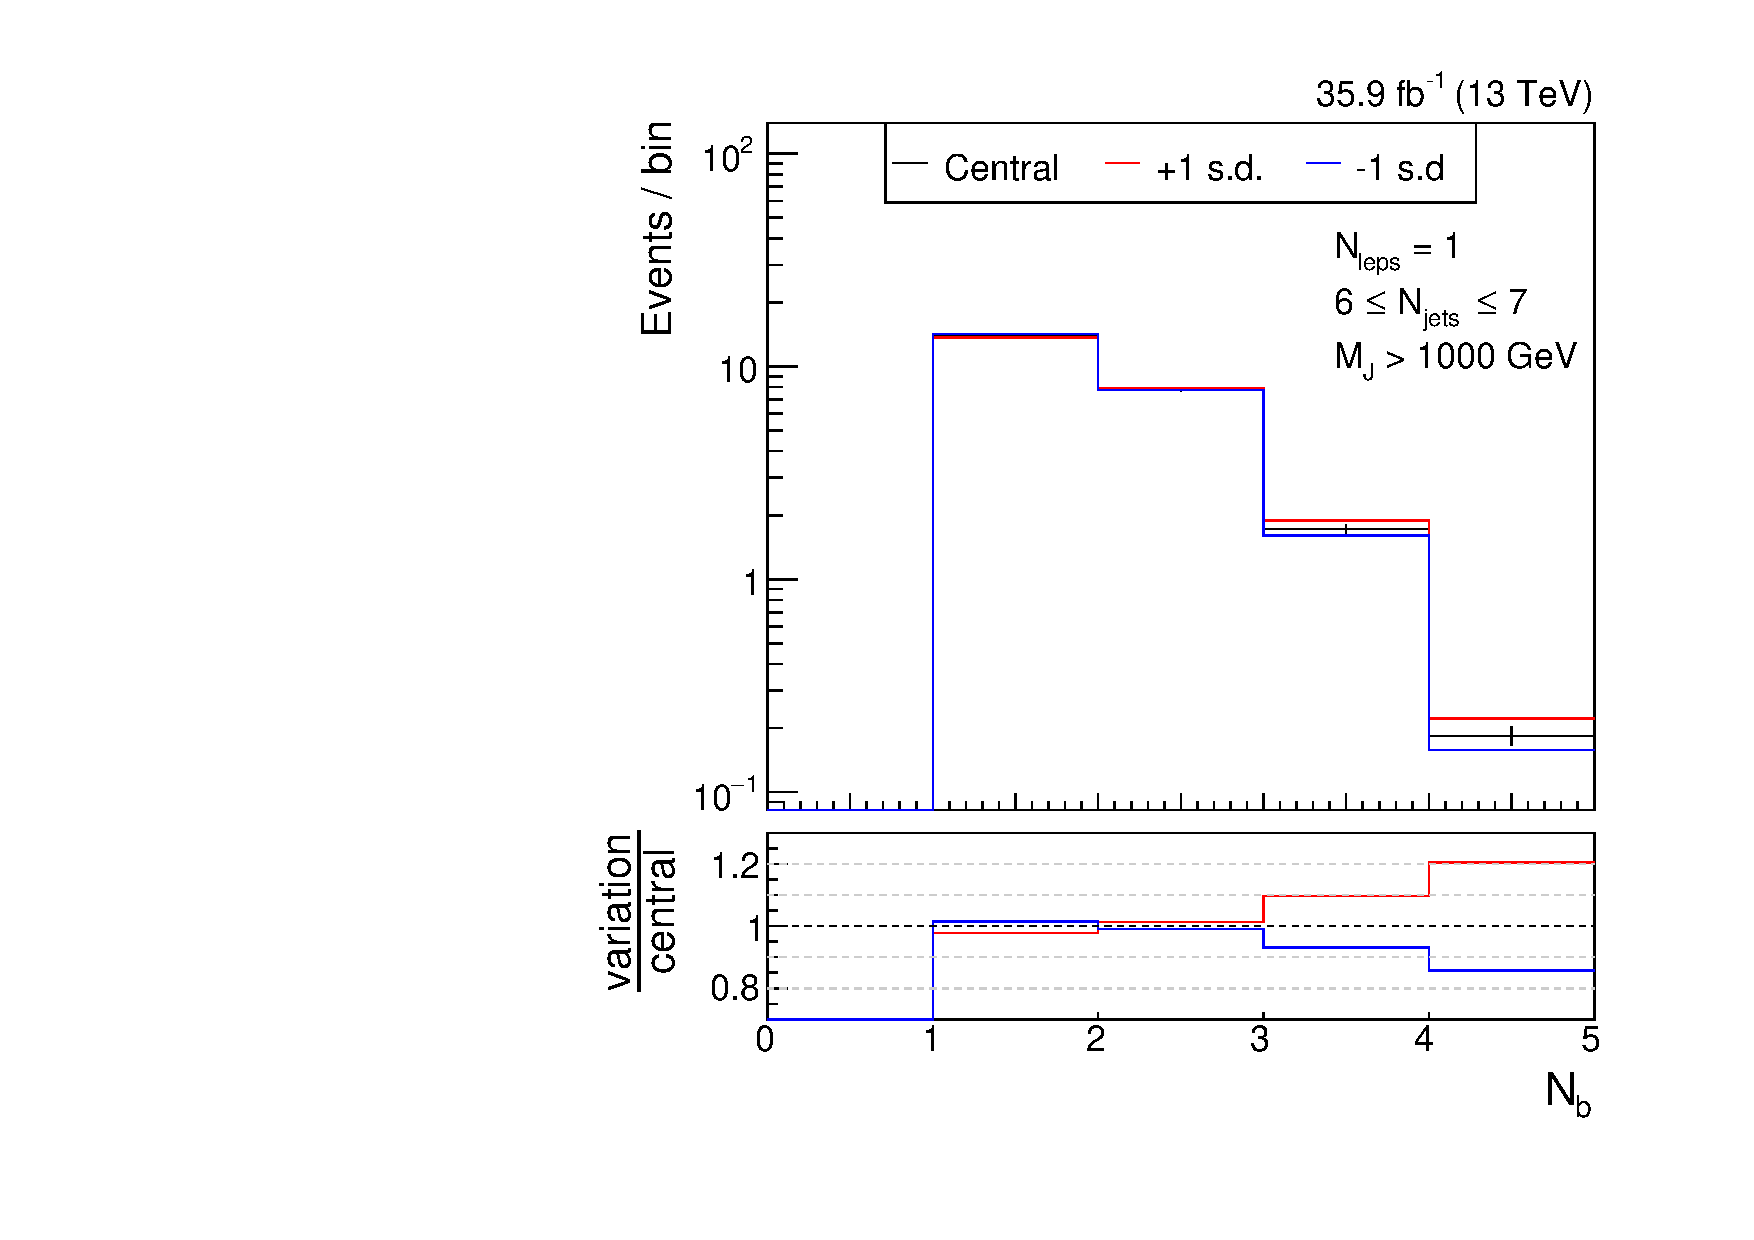
\includegraphics[angle=0,width=0.45\columnwidth]{fig/bin20_ttbar_gs_mconly.pdf}
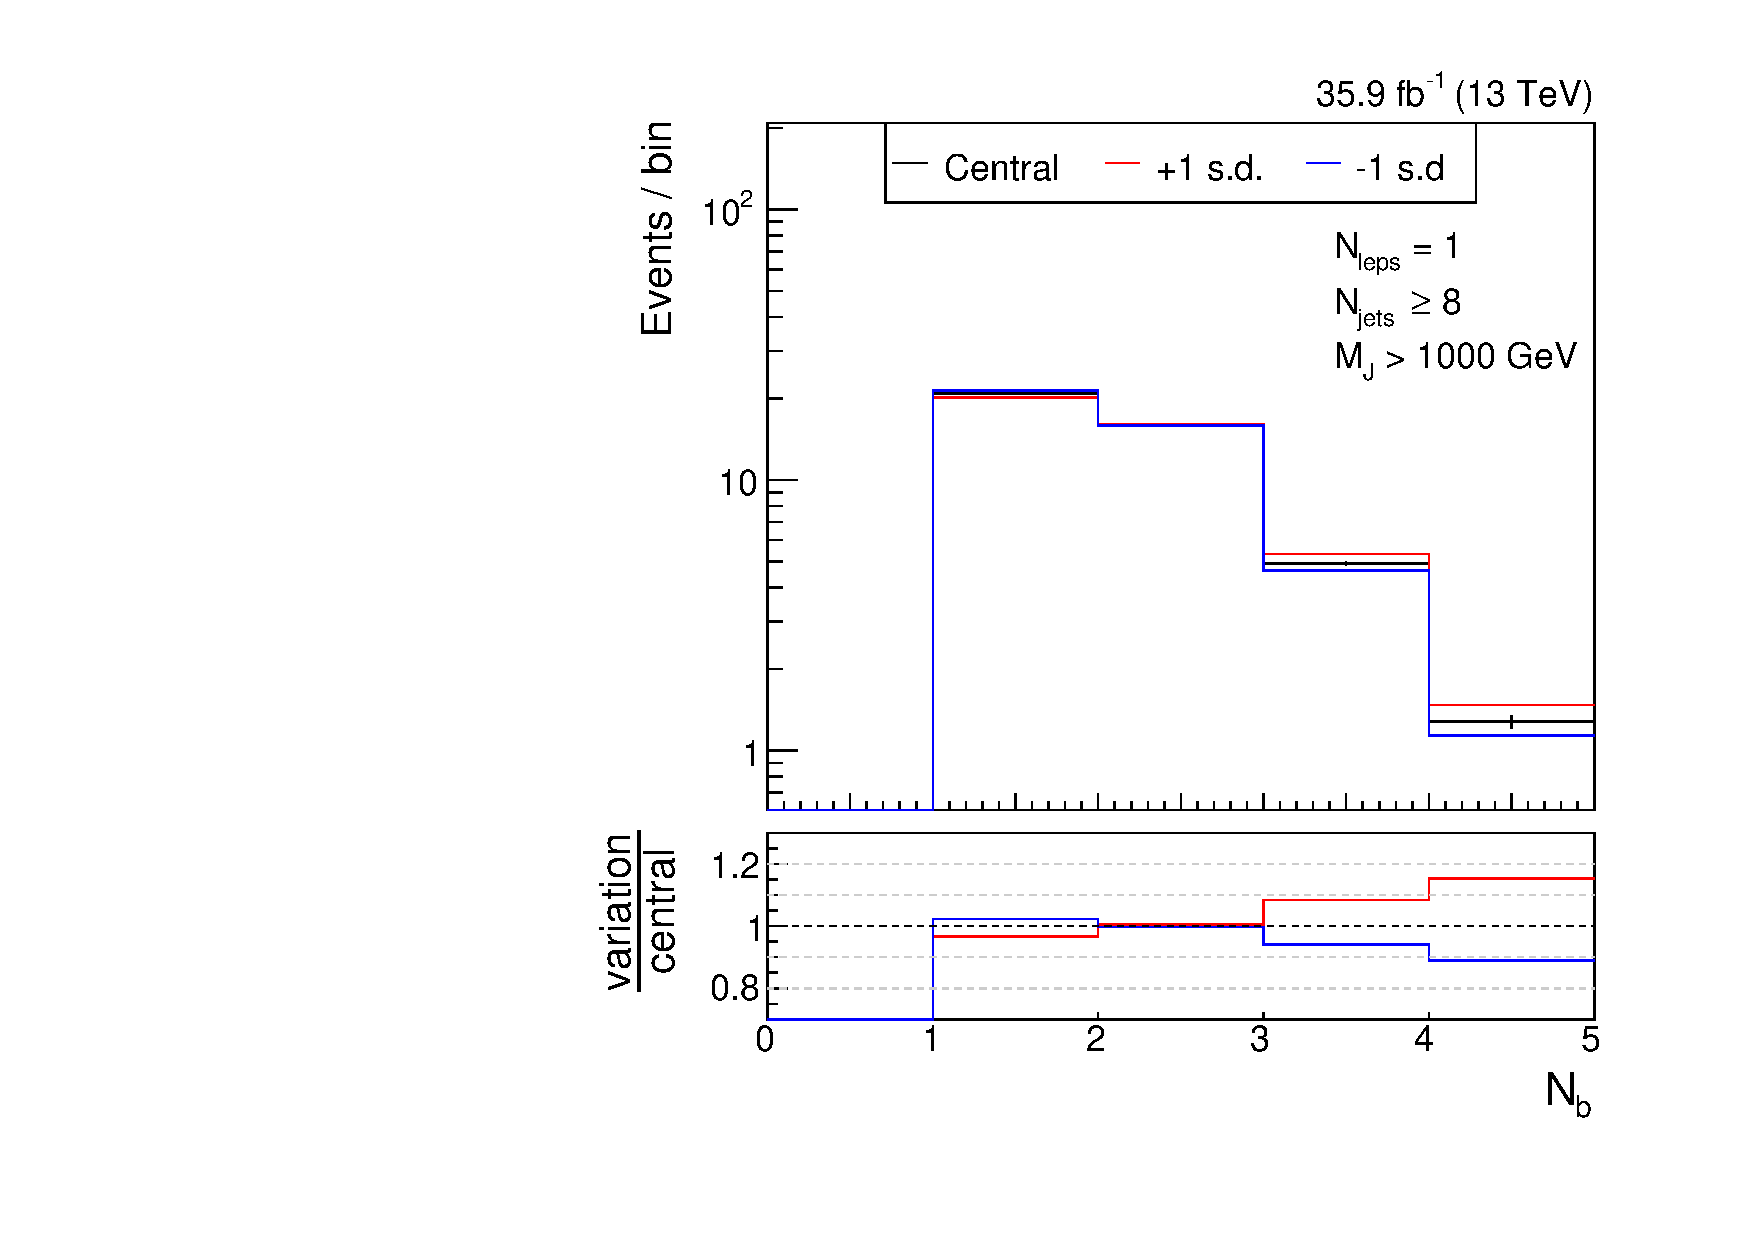
\includegraphics[angle=0,width=0.45\columnwidth]{fig/bin21_ttbar_gs_mconly.pdf}
\end{center}
\caption{Effect of the $\pm 1$~s.d.\ variations of the gluon splitting rate on the \Nb distribution in \ttbar events for the two most sensitive bins: $\Njets \geq 8$, $800 < \MJ \leq 1000~\GeV$ (left) and $\Njets \geq 8$, $\MJ > 1000~\GeV$ (right).
Event yields are normalized to that expected in $35.9~\ifb$ of data.}
\label{fig:gs_variations}
\end{figure}

In order to test the stability of the fit results and the dependence of the gluon splitting weights across kinematic regions, the \dRbb fit is repeated both with a higher \MJ threshold and with different \Njets bins. 
The resulting weights are shown in Table~\ref{tab:gs_variations} and are all consistent with those of the nominal fit.

\begin{table}[tb!]
\setlength\tabcolsep{3pt}
\centering
\begin{tabular}{l|cccccc}
 & Nominal & $\MJ > 800~\GeV$ & $4 \leq \Njets \leq 5$ & $6 \leq \Njets \leq 7$ & $8 \leq \Njets \leq 9$ & $\Njets \geq 10$ \\
\hline
GS    & $0.77 \pm 0.09$ & $0.70 \pm 0.38$ & $ 0.80 \pm 0.32$  & $ 0.76 \pm 0.14$ & $ 0.75 \pm 0.16$  & $ 0.95 \pm 0.36$ \\
No GS & $1.21 \pm 0.08$ & $1.28 \pm 0.35$ & $ 1.15 \pm 0.26$  & $ 1.22 \pm 0.13$ & $ 1.24 \pm 0.15$  & $ 1.05 \pm 0.36$ \\
\end{tabular}
\caption{Gluon splitting weights derived in the nominal fit, a variation with a requirement of $\MJ > 800~\GeV$, and 4 variations in bins of \Njets (with the nominal $\MJ > 500~\GeV$ requirement.)}
\label{tab:gs_variations}
\end{table}

\end{section}

\begin{section}{b-tagging Data-to-simulation Scale Factors}
\label{sec:btag_sfs}

Another significant systematic uncertainty is the uncertainty in the data-to-simulation scale factors (SF) for b~tagging efficiency and mistag rates.
Simulating the b-tagging algorithm relies on understanding the detailed behavior of the detector and also accurate modelling of the parton shower and hadronization, both of which are non-trivial.
Therefore, it is important to measure the b~tagging efficiencies and mistag rates in data and correct the simulation to match.

The difference between data and simulation is corrected for by using a per jet data-to-simulation SF
\begin{align}
SF_{f} = \varepsilon^{data}_{f}(\pT)/\varepsilon^{sim}_{f}(\pT).
\end{align}
where $\varepsilon^{data}_{f}(\pT)$ and $\varepsilon^{sim}_{f}(\pT)$ are the tagging efficiencies for a jet with flavor $f$ as a function of \pT in data and simulation, respectively.
No dependence on $\eta$ is derived due to limited data sample sizes.
In simulation, the efficiency is determined by matching jets to their generated hadron to determine their flavor and then measuring how many of those jets are correctly tagged.
In data, this is done by using control regions determined by specific selection requirements that produce pure samples of a certain flavor of jets while not biasing the jets with respect to variables used in the b~tagging algorithm.

The probability to tag a light-flavor or gluon jet (light jet) is measured in an inclusive QCD sample.
This sample is selected through a series of triggers that require at least one jet over a certain \pT threshold, the lowest being $40~\GeV$.

The probability to tag a charm-flavor jet (c jet) is determined by measurements in two charm-enriched control regions.
The first control region is formed by selecting events in which a charm quark is produced in association with a W boson.
The main contributions to this process is from $\mrm{s} + \mrm{g} \to \mrm{W^{-}} + \mrm{c}$ and $\mrm{\bar{s}} + \mrm{g} \to \mrm{W^{+}} + \mrm{\bar{c}}$, where a key property is that the W boson and quark have oppositely signed electrical charges.
The dominant background is $\mrm{W} + \mrm{q\bar{q}}$ events, which produce an equal amount of events with same- and opposite-signed W boson and quark pairs.
Thus, this background is removed by measuring its contribution in the same-sign channel and then subtracting it from the opposite-sign channel, resulting in a pure $\mrm{W} + \mrm{c}$ channel.
The second charm-enriched control region is created by selecting single-lepton \ttbar events.
As hadronically-decaying W bosons decay to a charm quark about 50\% of the time, about one of two single-lepton \ttbar events will contain a charm quark.
Finally, measurements in these two regions are combined using the best linear unbiased estimator (BLUE) method described in Reference~\cite{LYONS1988110}.

The probability to tag a b-flavor jet (b jet) is computed using QCD and \ttbar control regions.
The QCD control regions are enriched in b quarks by requiring that at least one jet contains a muon with $\pT > 5~\GeV$, which takes advantage of the high branching fraction to leptons of b hadrons.
In the \ttbar-dominated regions, there are two b quarks per event, due to the decay of the two top quarks, and the b quark purity is further enhanced by limiting the number of non-b jets in the event through the requirement that either one or both of the W bosons decays leptonically.
This creates independent single-lepton and di-lepton control regions where multiple measurements are made and then combined through the BLUE method.

The resulting SFs, including their uncertainties, are shown in Figure~\ref{fig:btag_sfs}.
A complete discussion of how the SF measurements are made can be found in Reference~\cite{Sirunyan:2017ezt}.

\begin{figure}[tbp!]
\begin{center}
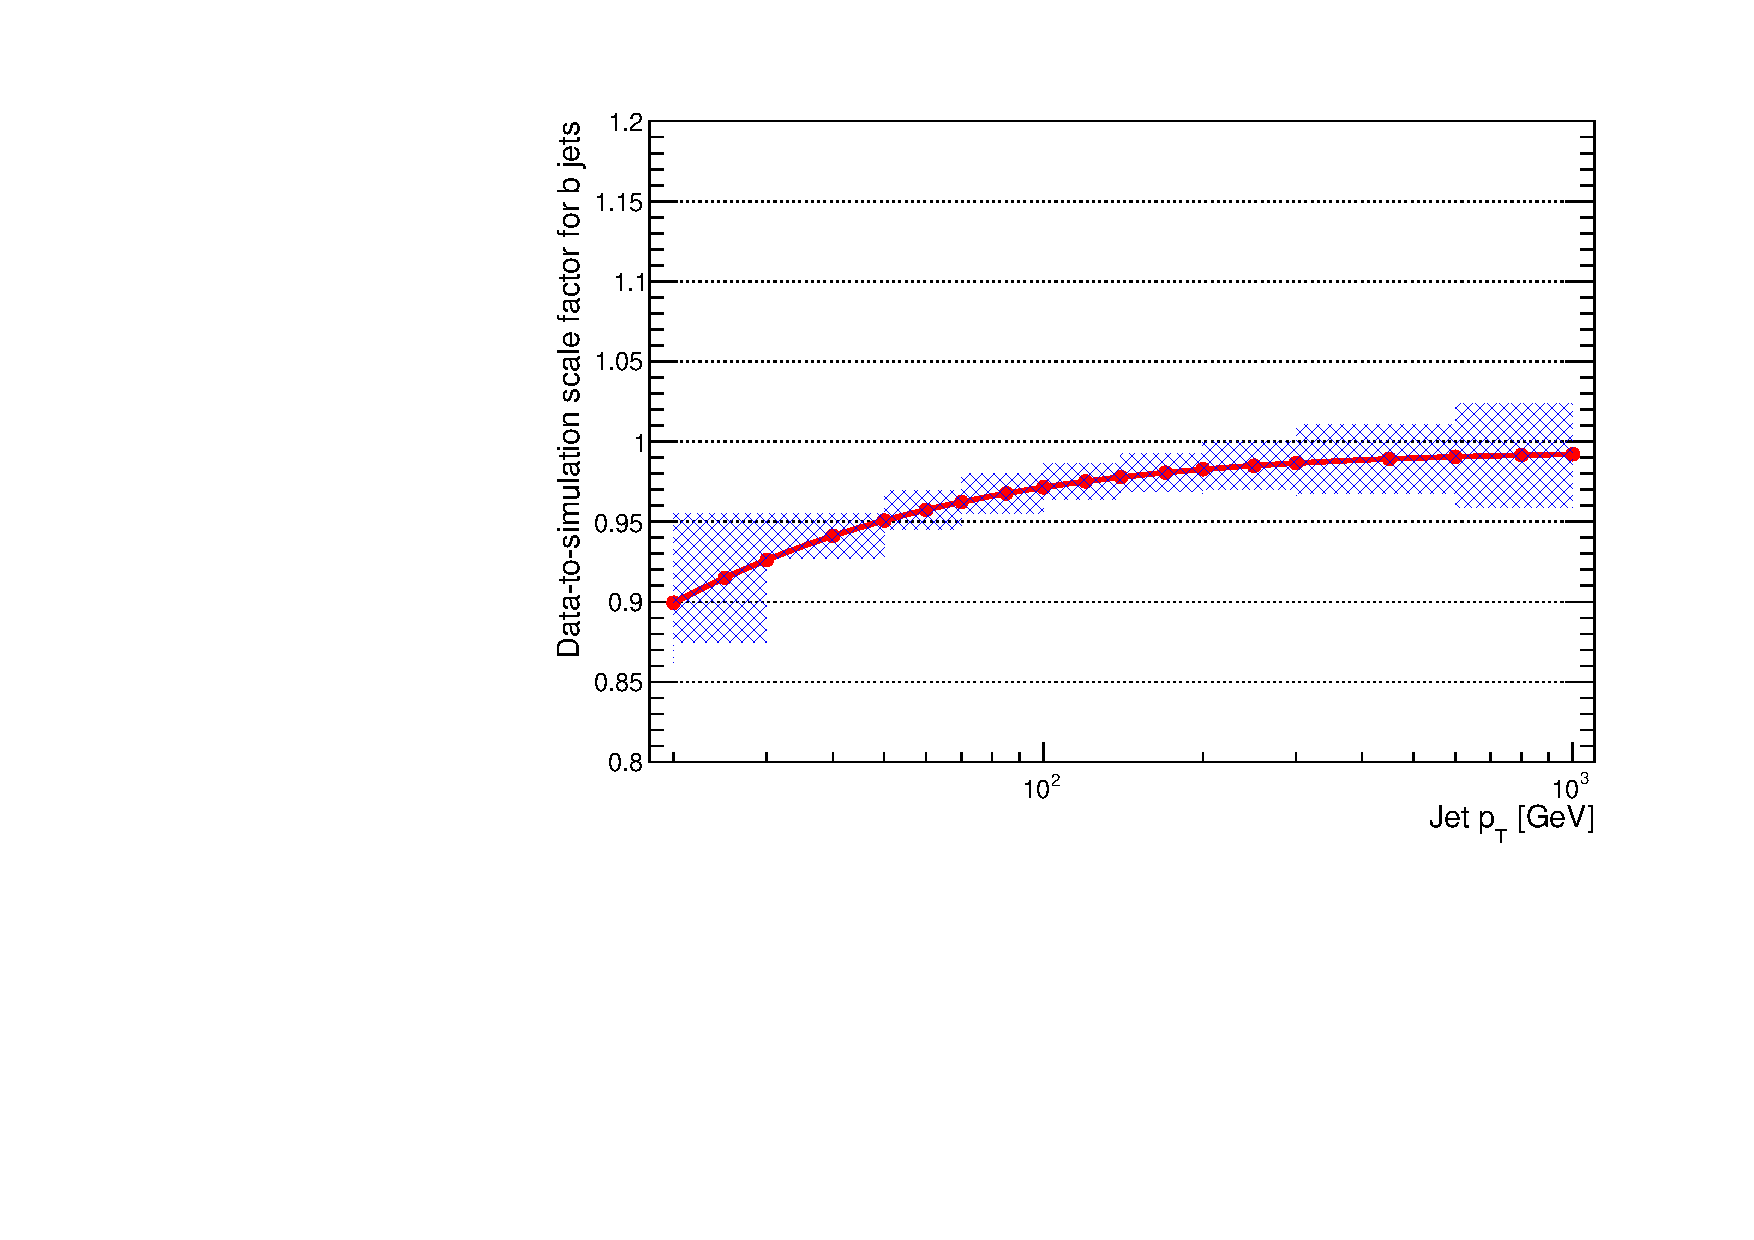
\includegraphics[angle=0,width=0.48\columnwidth]{fig/sfs_bjet.pdf}
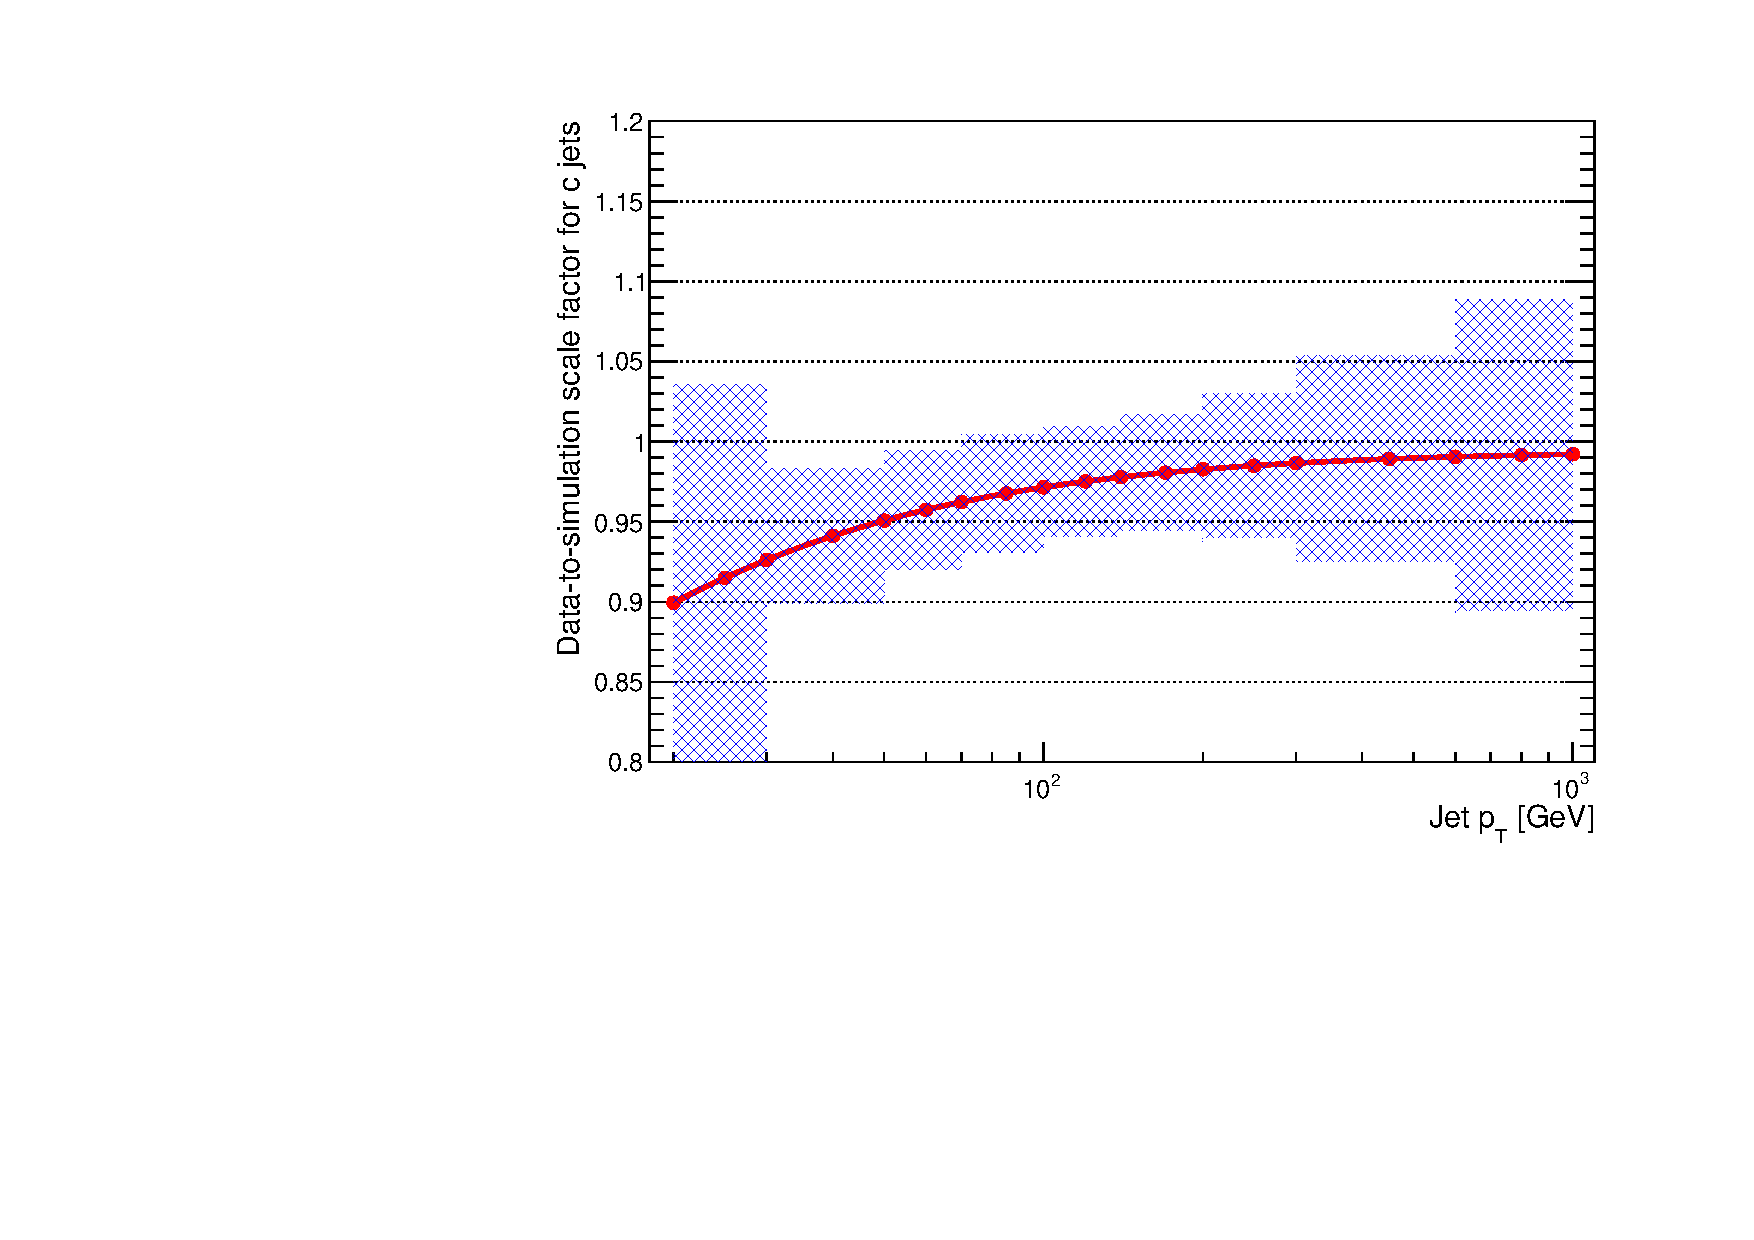
\includegraphics[angle=0,width=0.48\columnwidth]{fig/sfs_cjet.pdf}
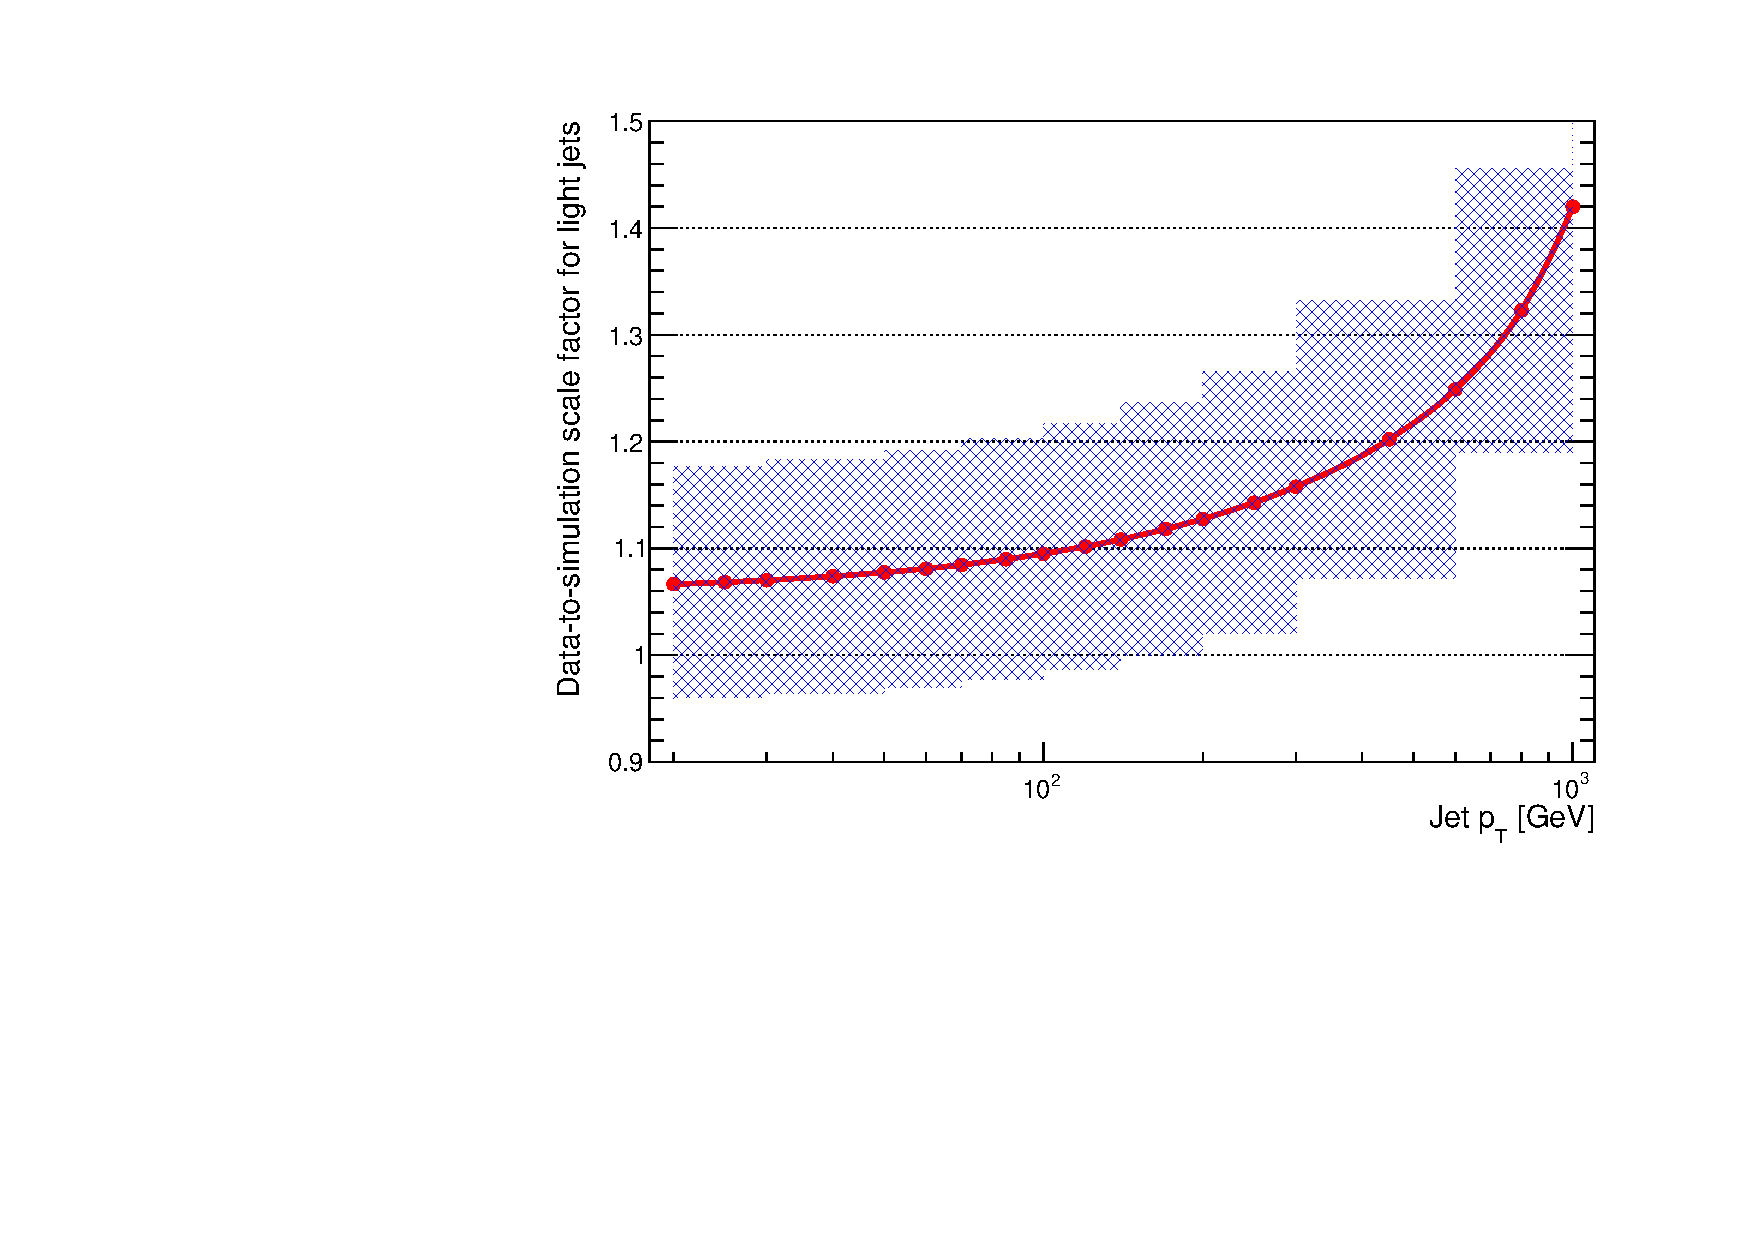
\includegraphics[angle=0,width=0.48\columnwidth]{fig/sfs_ljet.pdf}
\end{center}
\caption{The data-to-simulation scale factors for the tagging efficiency of b-flavor jets (top-left), charm-flavor jets (top-right), and light-flavor or gluon jets (bottom) are shown as a function of jet \pT.
The associated uncertainty with each scale factor is shown as a blue hashed band.}
\label{fig:btag_sfs}
\end{figure}

The systematic uncertainties on the \Nb shape are assessed by the $\pm 1$~s.d.\ \Nb templates resulting from varying the SFs according to their uncertainties.
Because the b and c jet SFs have correlated uncertainties, they are conservatively varied together and form one set of templates.
The light-flavor SFs are uncorrelated with the b and c jet SFs and are varied independently.
The effects of these variations on the \Nb distribution in \ttbar events are shown in Figure~\ref{fig:sf_bc_variations} and Figure~\ref{fig:sf_udsg_variations}.

\begin{figure}[tbp!]
\begin{center}
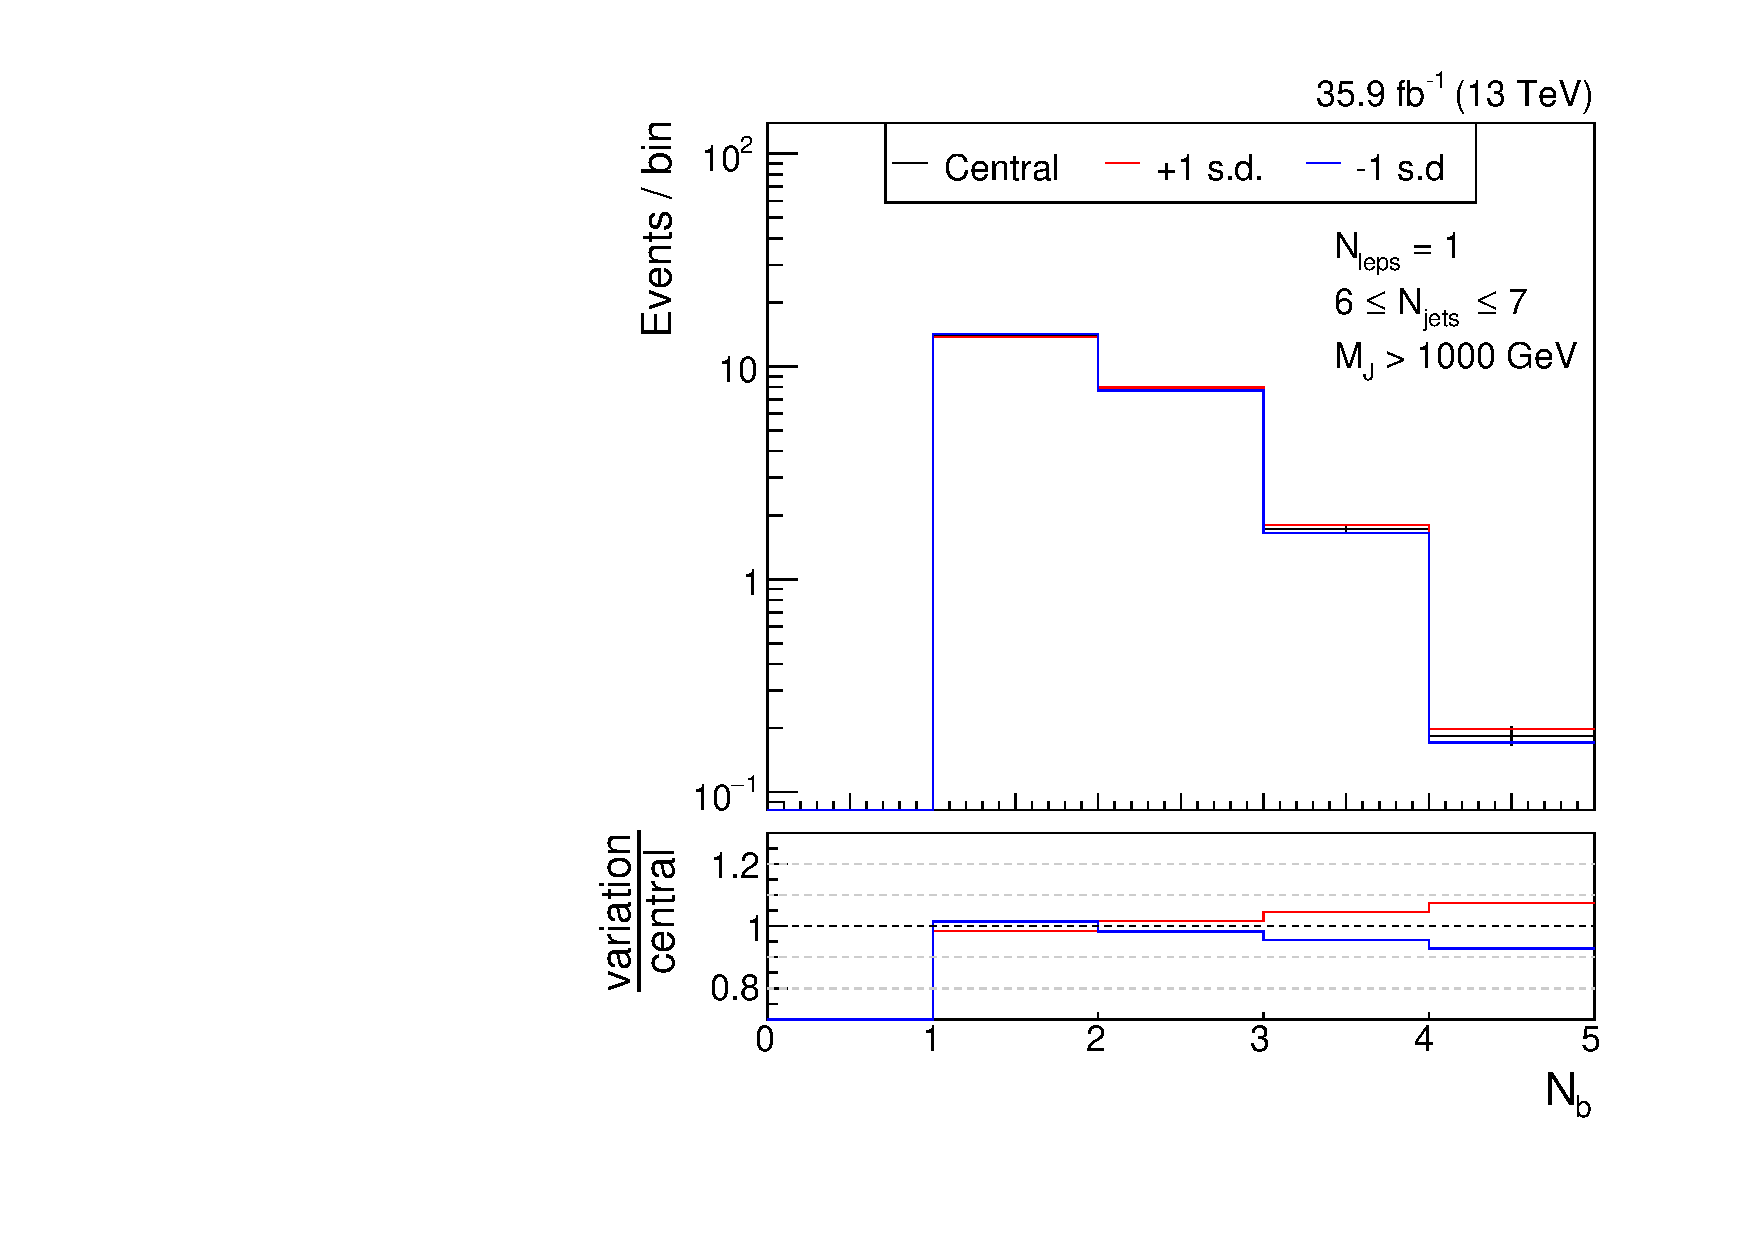
\includegraphics[angle=0,width=0.45\columnwidth]{fig/bin20_ttbar_btag_bc_mconly.pdf}
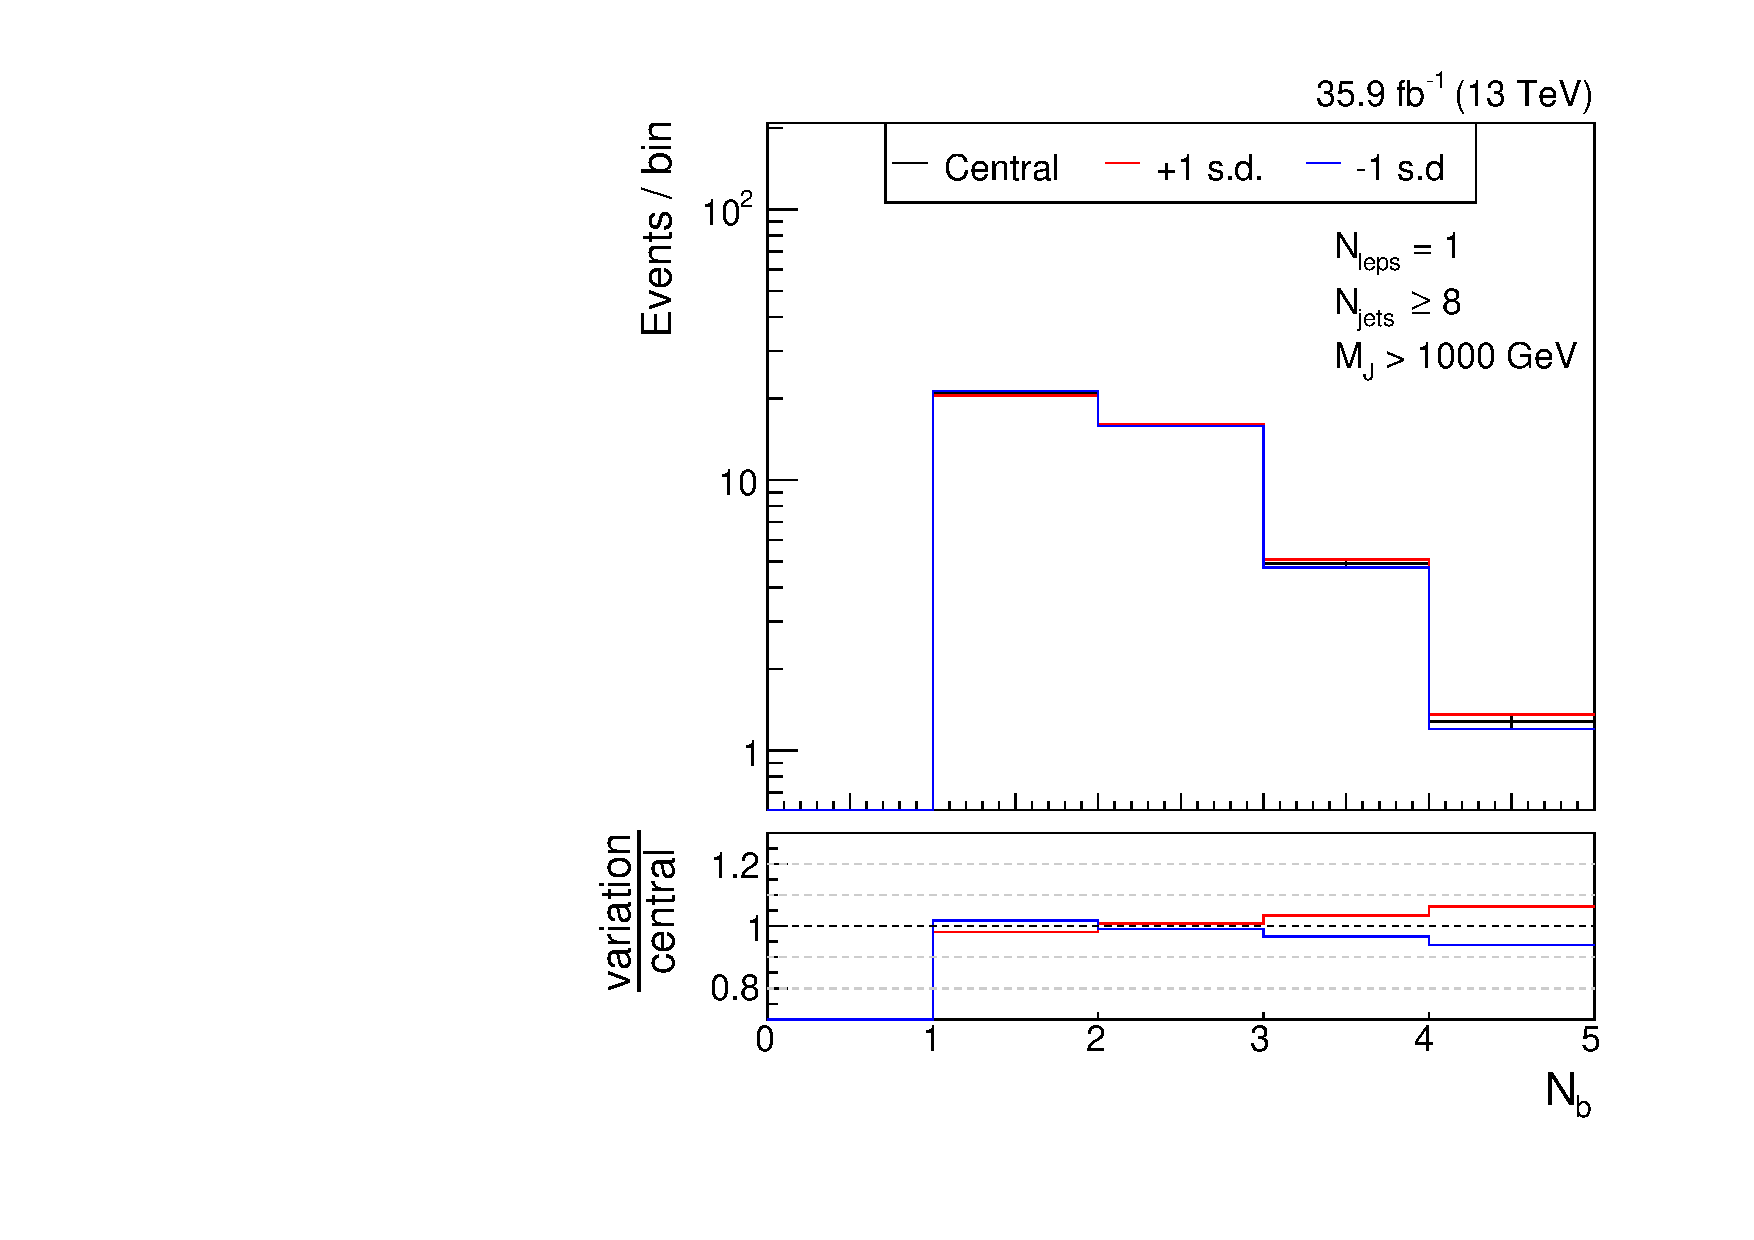
\includegraphics[angle=0,width=0.45\columnwidth]{fig/bin21_ttbar_btag_bc_mconly.pdf}
\end{center}
\caption{Effect of the $\pm 1$~s.d.\ correlated variations of the b-flavor and c-flavor jet data-to-simulation scale factors on the \Nb distribution in \ttbar for the two most sensitive bins: $\Njets \geq 8$, $800 < \MJ \leq 1000~\GeV$ (left) and $\Njets \geq 8$, $\MJ > 1000~\GeV$ (right).
Event yields are normalized to that expected in $35.9~\ifb$ of data.}
\label{fig:sf_bc_variations}
\end{figure}

\begin{figure}[tbp!]
\begin{center}
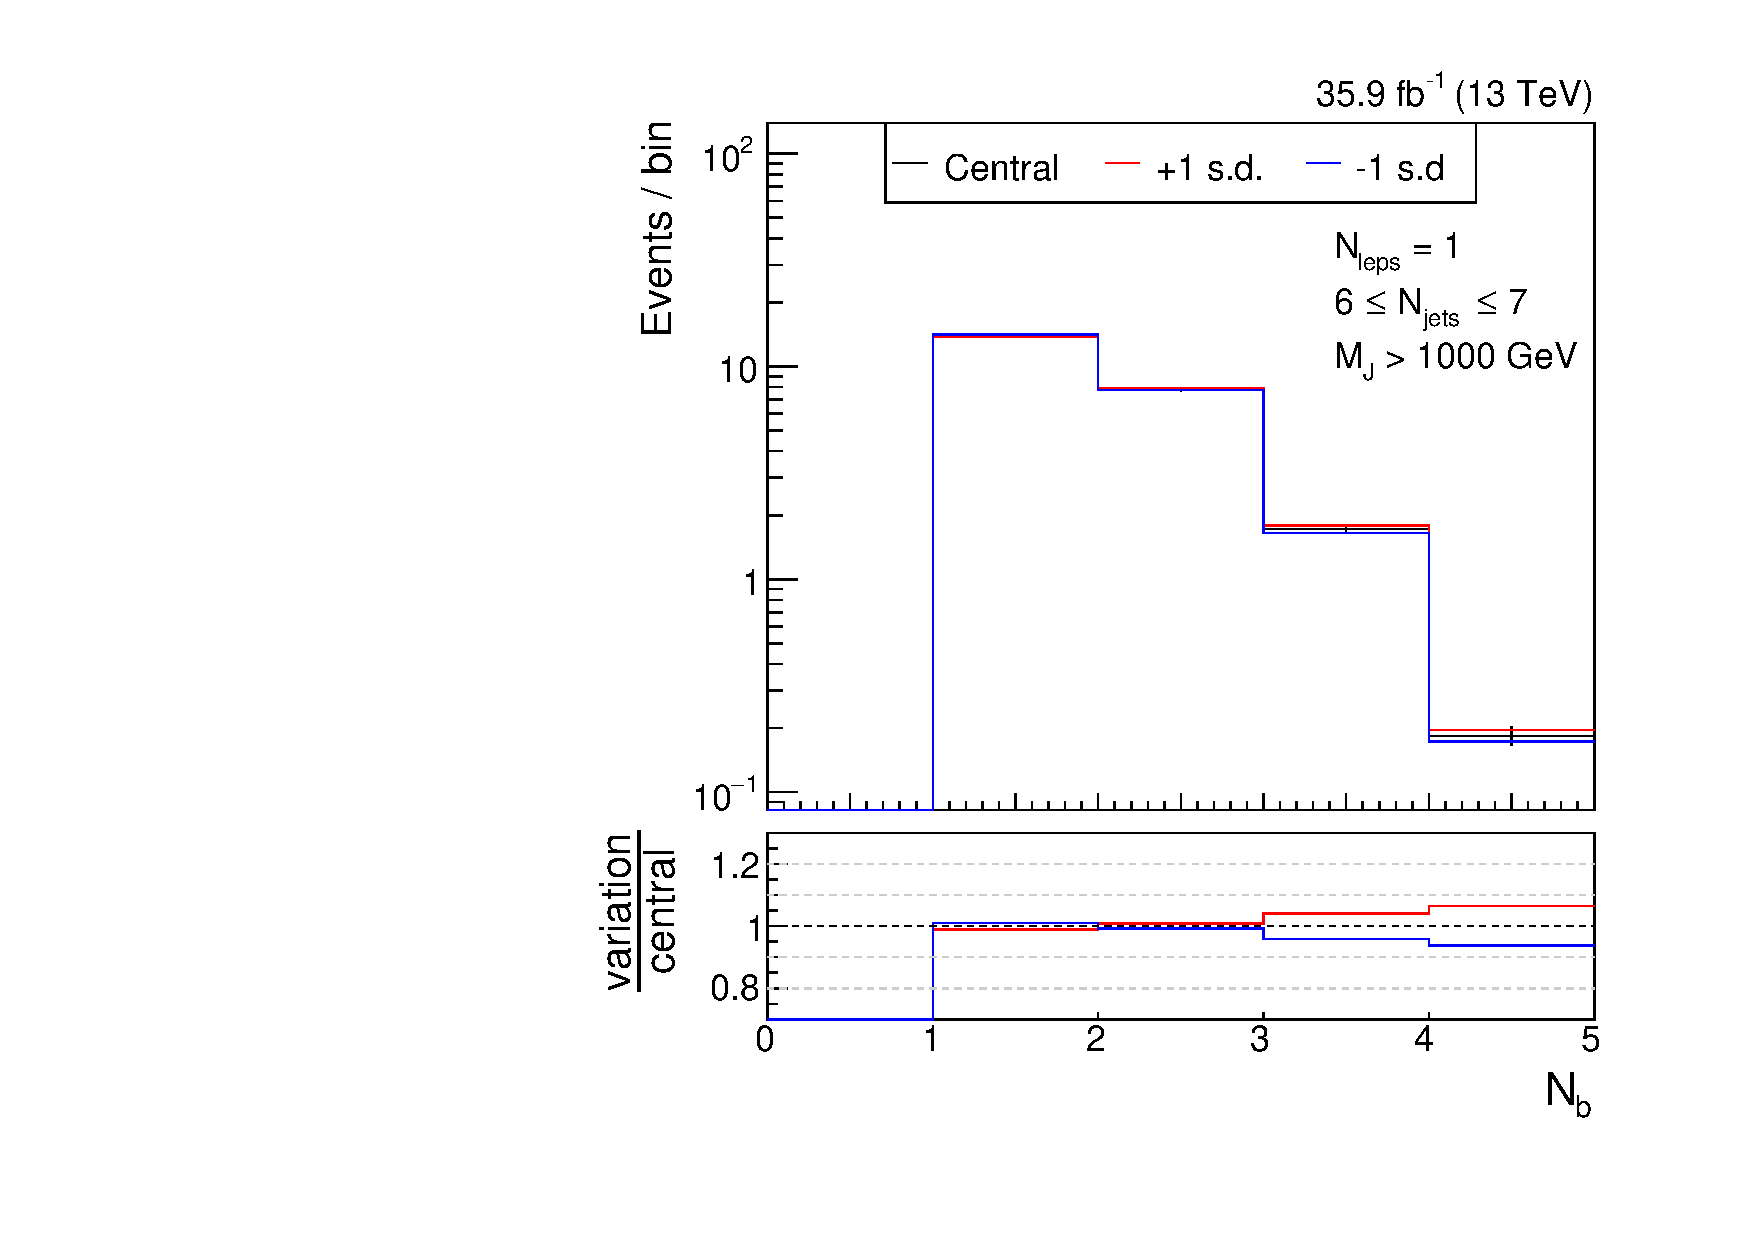
\includegraphics[angle=0,width=0.45\columnwidth]{fig/bin20_ttbar_btag_udsg_mconly.pdf}
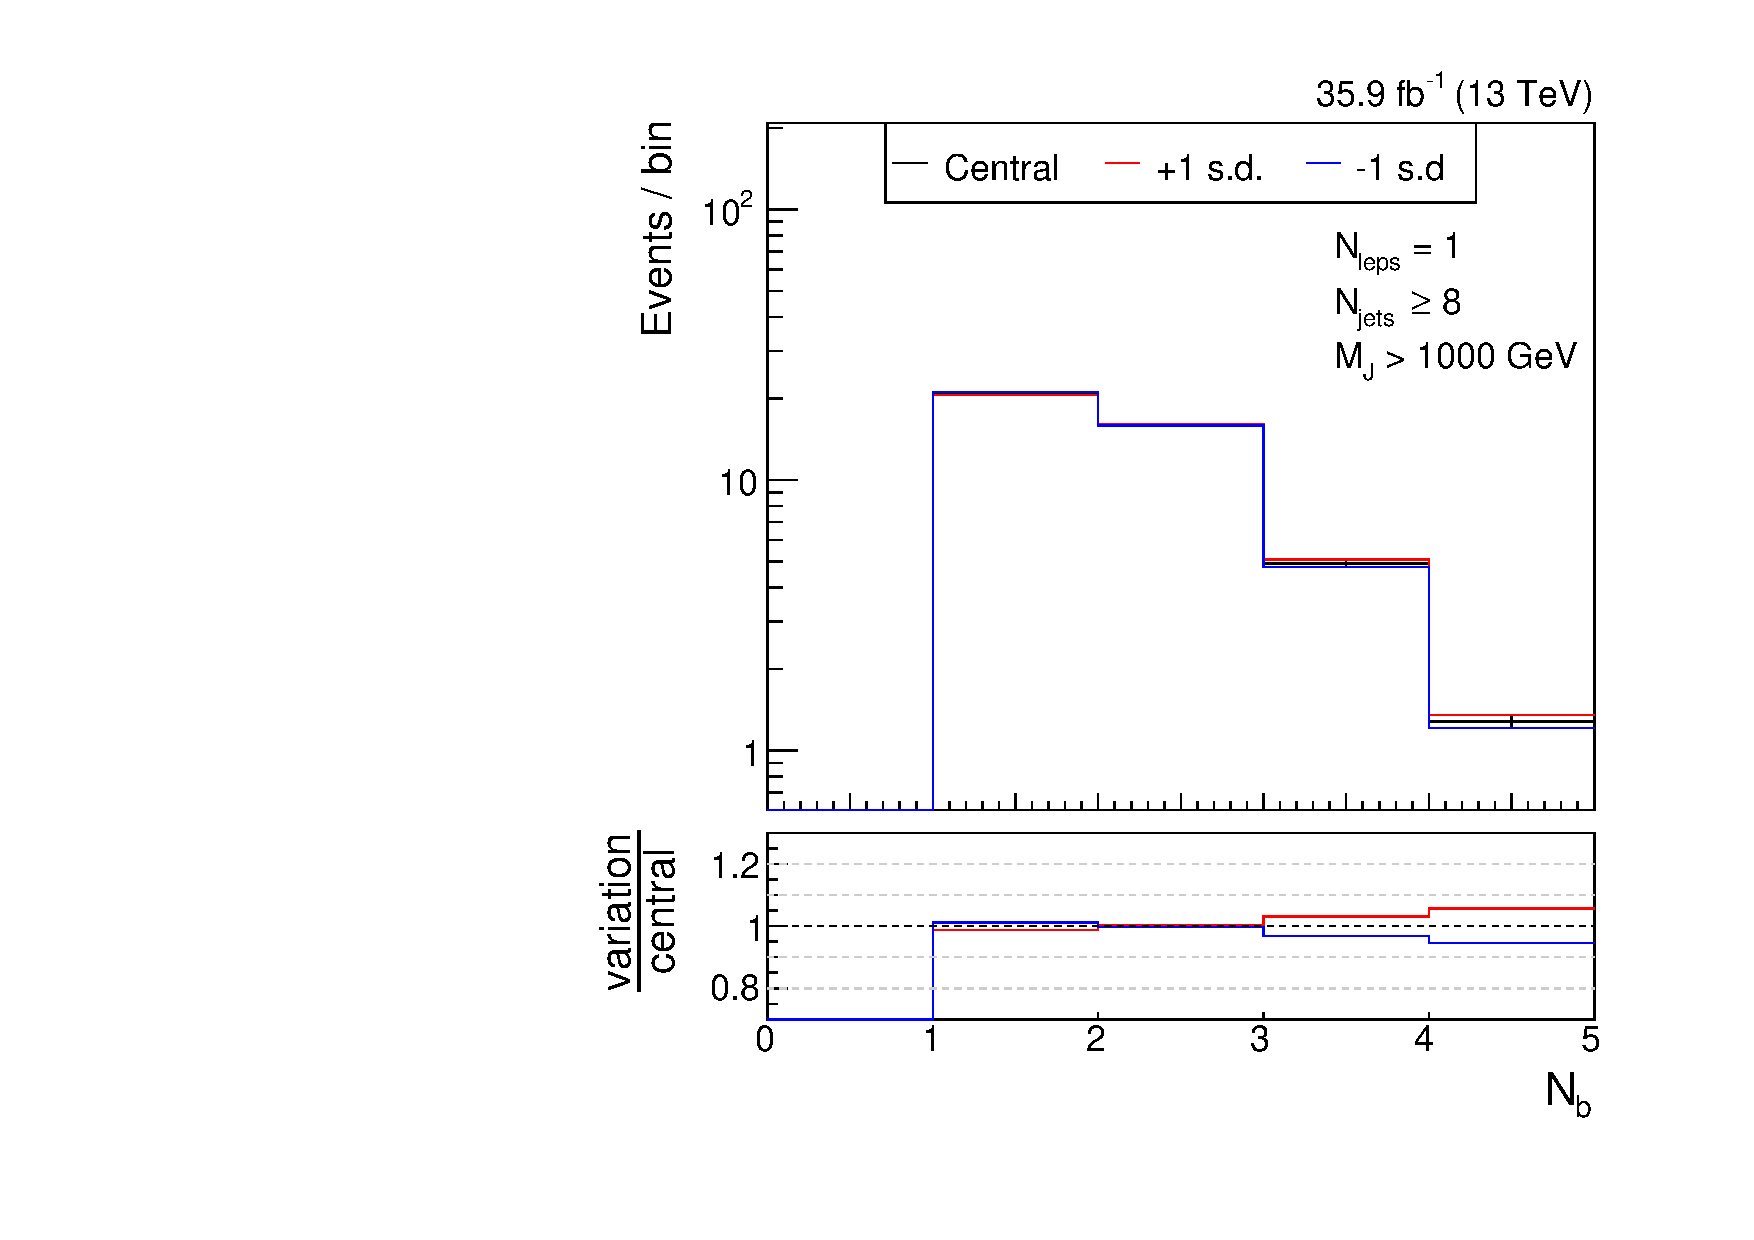
\includegraphics[angle=0,width=0.45\columnwidth]{fig/bin21_ttbar_btag_udsg_mconly.pdf}
\end{center}
\caption{Effect of the $\pm 1$~s.d.\ variations of the light-flavor jet data-to-simulation scale factors on the \Nb distribution in \ttbar for the two most sensitive bins: $\Njets \geq 8$, $800 < \MJ \leq 1000~\GeV$ (left) and $\Njets \geq 8$, $\MJ > 1000~\GeV$ (right).
Event yields are normalized to that expected in $35.9~\ifb$ of data.}
\label{fig:sf_udsg_variations}
\end{figure}

\end{section}

\begin{section}{Lepton Fake Rate in QCD}

While the QCD normalization is measured from data, it is mostly constrained by the $\Nleps = 0$ selection and applied in a $\Nleps = 1$ region.
If the simulated \Nleps distribution is not modelled perfectly, there may be residual differences between the normalizations of these two regions.
For processes that have true prompt leptons, such as \ttbar and \Wjets, the \Nleps distribution is well modelled, because the dominant effects are the W branching fractions and the acceptance (including selection efficiency), both of which are well understood. 
For QCD, however, this is less well modelled as the simulation of the tail of the jet fragmentation function, as well as detector effects that can produce fake leptons, are not as well understood.

To assign a systematic uncertainty on the modelling of the ratio of 0-lepton to 1-lepton events in QCD, the lepton isolation distributions are studied.
Figure~\ref{fig:lep_iso} shows the relative isolation distributions for eletrons (left) and muons (right) in a data sample corresponding to the analysis control regions.
The binning of the histograms are chosen such that the first bin corresponds to the relative isolation requirement for signal leptons (0.1 for electrons and 0.2 for muons).
The normalizations of the QCD, \ttbar, and \Wjets processes are scaled to match the results of a control region fit described in Section~\ref{subsec:crfit}.

\begin{figure}[tbp!]
\begin{center}
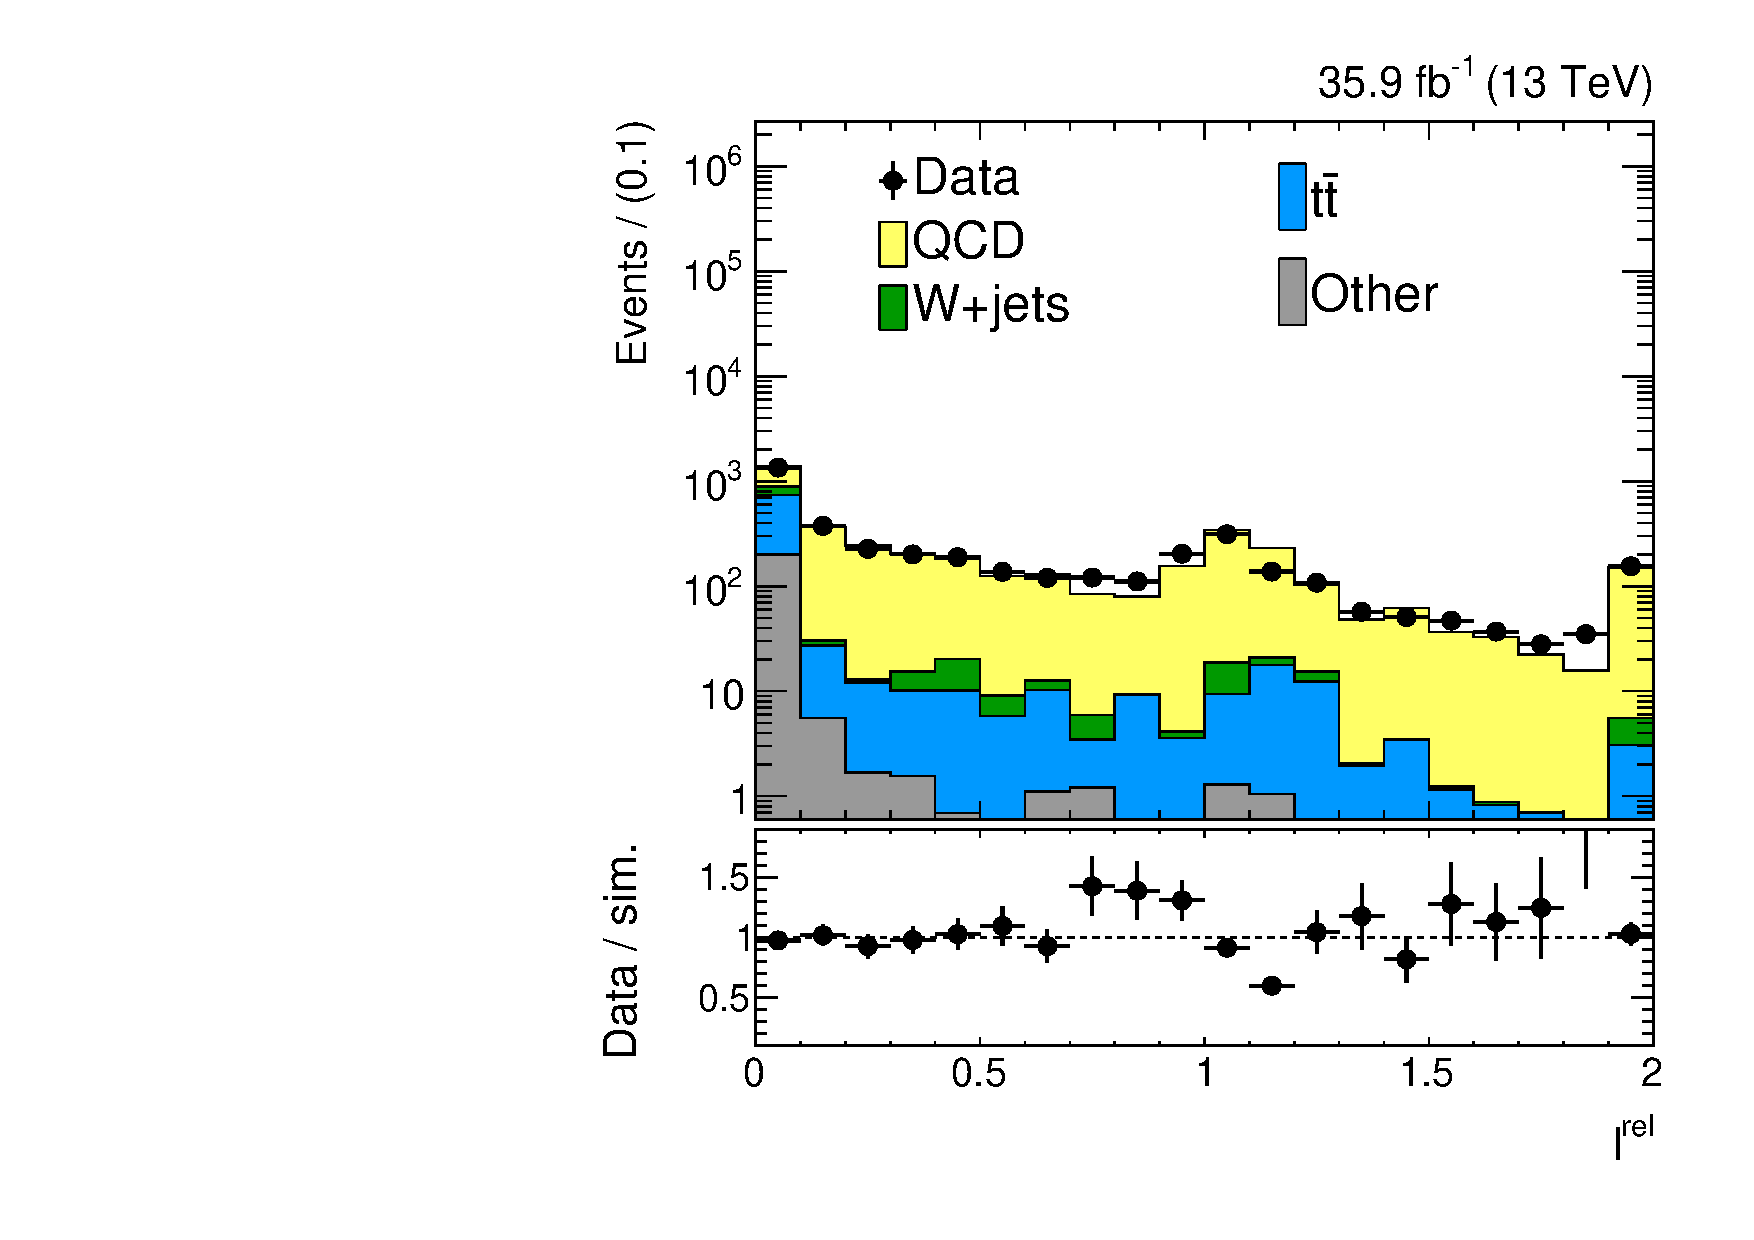
\includegraphics[angle=0,width=0.45\columnwidth]{fig/iso_els.pdf}
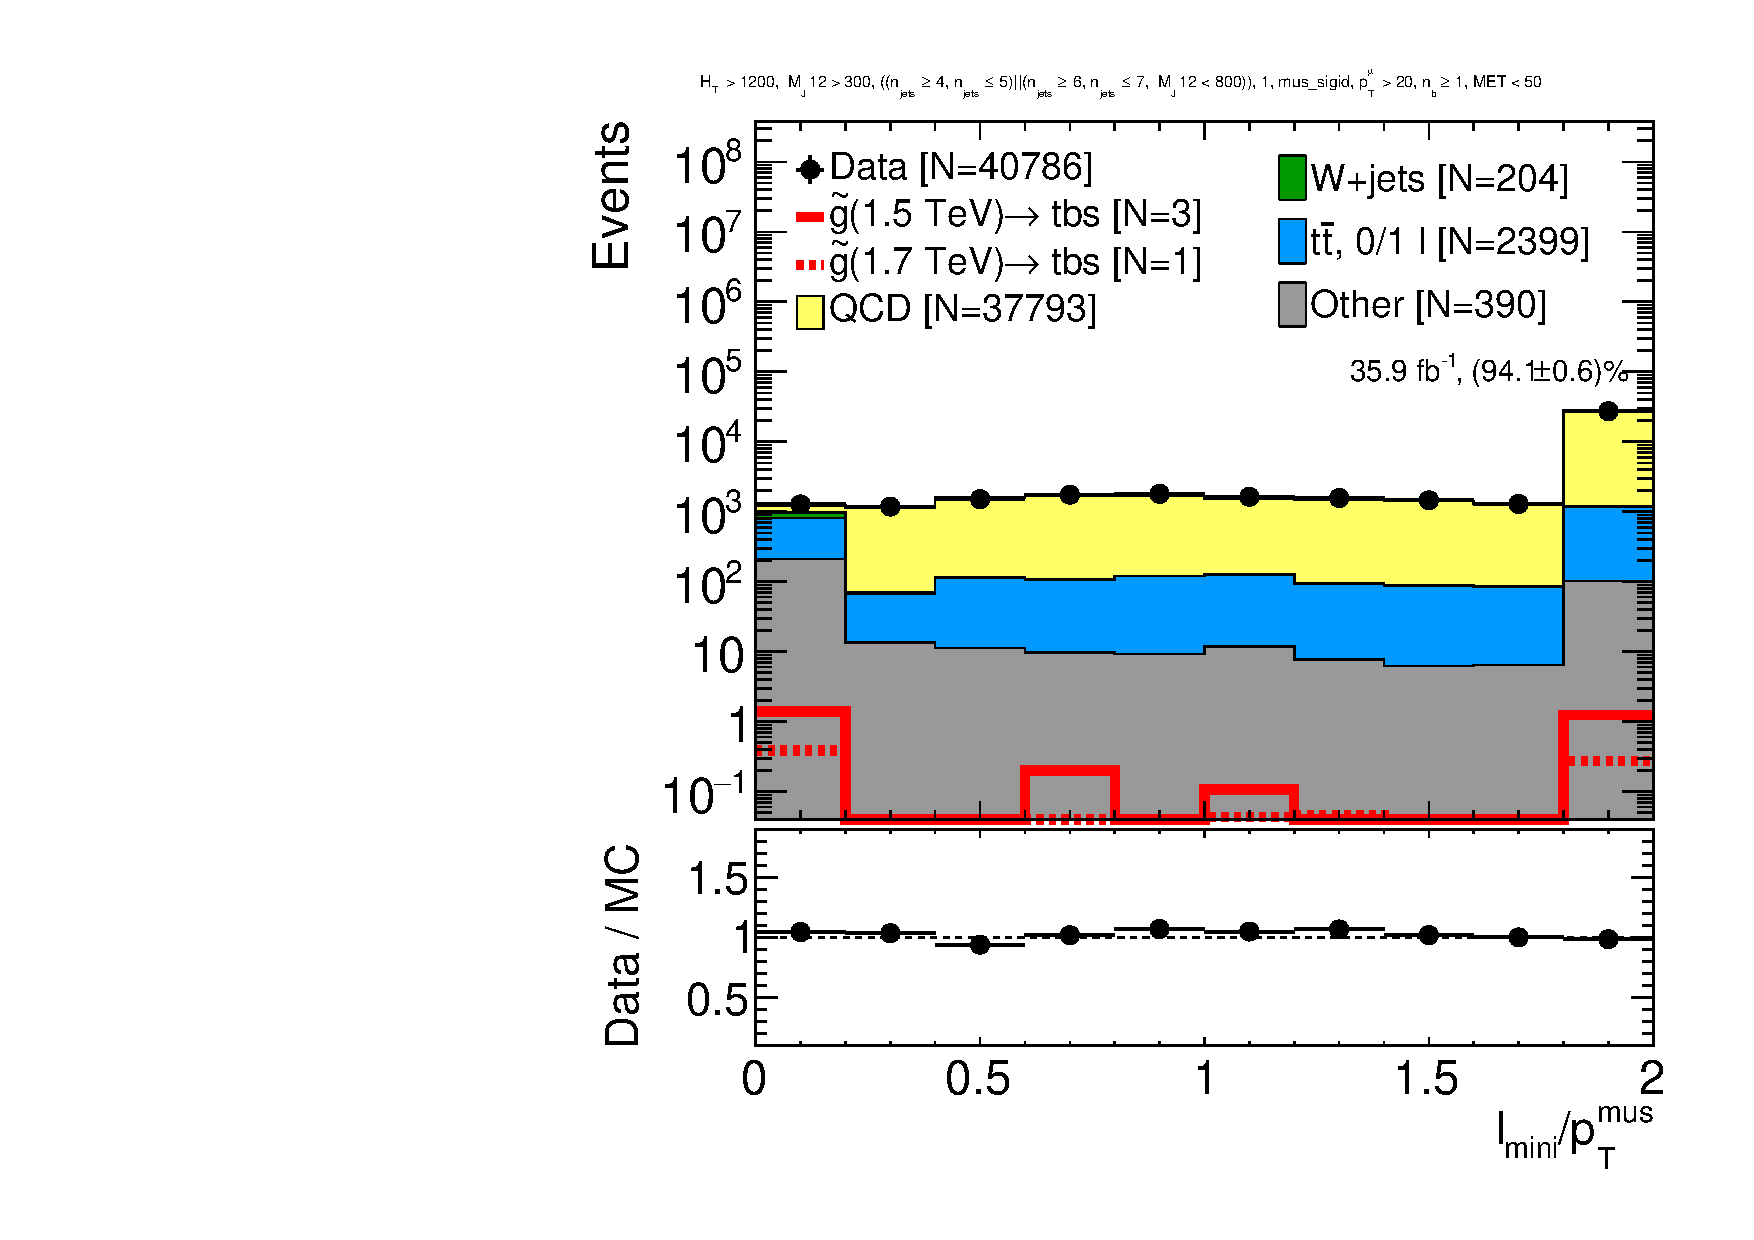
\includegraphics[angle=0,width=0.45\columnwidth]{fig/iso_mus.pdf}
\end{center}
\caption{The relative isolation distribution for electrons (left) and muons (right) in the analysis control region.
The binning of the histograms is chosen such that the first bin corresponds to the relative isolation requirement for signal leptons (0.1 for electrons and 0.2 for muons).
The normalizations of the QCD, \ttbar, and \Wjets processes are scaled to match the results of a control region fit described in Section~\ref{subsec:crfit}.}
\label{fig:lep_iso}
\end{figure}

Table~\ref{tab:lep_iso} shows the ratio of $I^{\mrm{rel}} < 0.1(0.2)$ to $I^{\mrm{rel}} \geq 0.1(0.2)$ for electrons(muons) in QCD and data with contributions for all other processes (\ttbar, \Wjets, Other) subtracted.
As the ratio in data agrees to that in QCD simulation within 20\%, an additional 20\% log-normal uncertainty is assigned to the QCD normalization, which is fully correlated across the 1-lepton bins.

\begin{table}[h]
\centering
\begin{tabular}{l | cc|c | cc|c }
\hline\hline
\multirow{2}{*}{Process}  &  \multicolumn{3}{c|}{Electrons}                                        &  \multicolumn{3}{c}{Muons}                                        \\
                          &  $I^{\mrm{rel}} < 0.1$          &  $I^{\mrm{rel}} \geq 0.1$  & ratio  &  $I^{\mrm{rel}} < 0.2$      &  $I^{\mrm{rel}} \geq 0.2$  &  ratio \\
\hline
QCD                       &  496.8                          &  2455.5                    &  0.20  &  219.8                      &  36553.3                   & 0.0060 \\
Data - all other          &  452.8                          &  2500.5                    &  0.18  &  275.4                      &  37497.7                   & 0.0073 \\
\hline\hline
\end{tabular}
\caption{Comparison of the relative isolation distributions, as described in the caption of Figure~\ref{fig:lep_iso}, for electrons and muons between QCD and data with contributions from ``all other'' (\ttbar, \Wjets, and Other) subtracted.}
\label{tab:lep_iso}
\end{table}

\end{section}

\begin{section}{Additional Systematic Uncertainties}

Other experimental uncertainties are small and include lepton selection efficiency, jet energy scale, jet energy resolution, and integrated luminosity.
The uncertainty associated with lepton selection efficiency is determined by varying the efficiency to select a lepton within its uncertainty determined from data.
Jet energy scale uncertainties~\cite{Chatrchyan:2011ds,1748-0221-12-02-P02014} are assessed by varying the \pT of small-$R$ jets as a function of \pT and $\eta$.
The uncertainty arising from jet energy resolution~\cite{Chatrchyan:2011ds,1748-0221-12-02-P02014} is determined by applying an $|\eta|$-dependent factor to the jet \pT to match the jet energy resolution observed in data.
The integrated luminosity is varied according to its uncertainty of 2.5\%~\cite{CMS-PAS-LUM-17-001}, affecting only the backgrounds estimated from simulation.
No uncertainty is applied for the amount of pileup as studies have shown its effect to be negligible in this high-\HT selection.
The uncertainties due to the limited size of simulation samples are incorporated as uncorrelated nuisance parameters in the fit.

Theoretical systematic uncertainties are applied and include independent and correlated variations of the renormalization  and factorization scales.
Additionally, uncertainties on the PDF are incorporated by considering variations in the NNPDF 3.0 scheme~\cite{Ball:2014uwa}.
The size of these uncertainties is typically small as the effect of these variations is largely to modify the cross section of processes, which for the main backgrounds are constrained by data.

The background systematic uncertainties that affect the \Nb shape are shown in Figure~\ref{fig:bkg_sys_tables} for the two most sensitive search bins.

\begin{figure}[tbp!]
\begin{center}
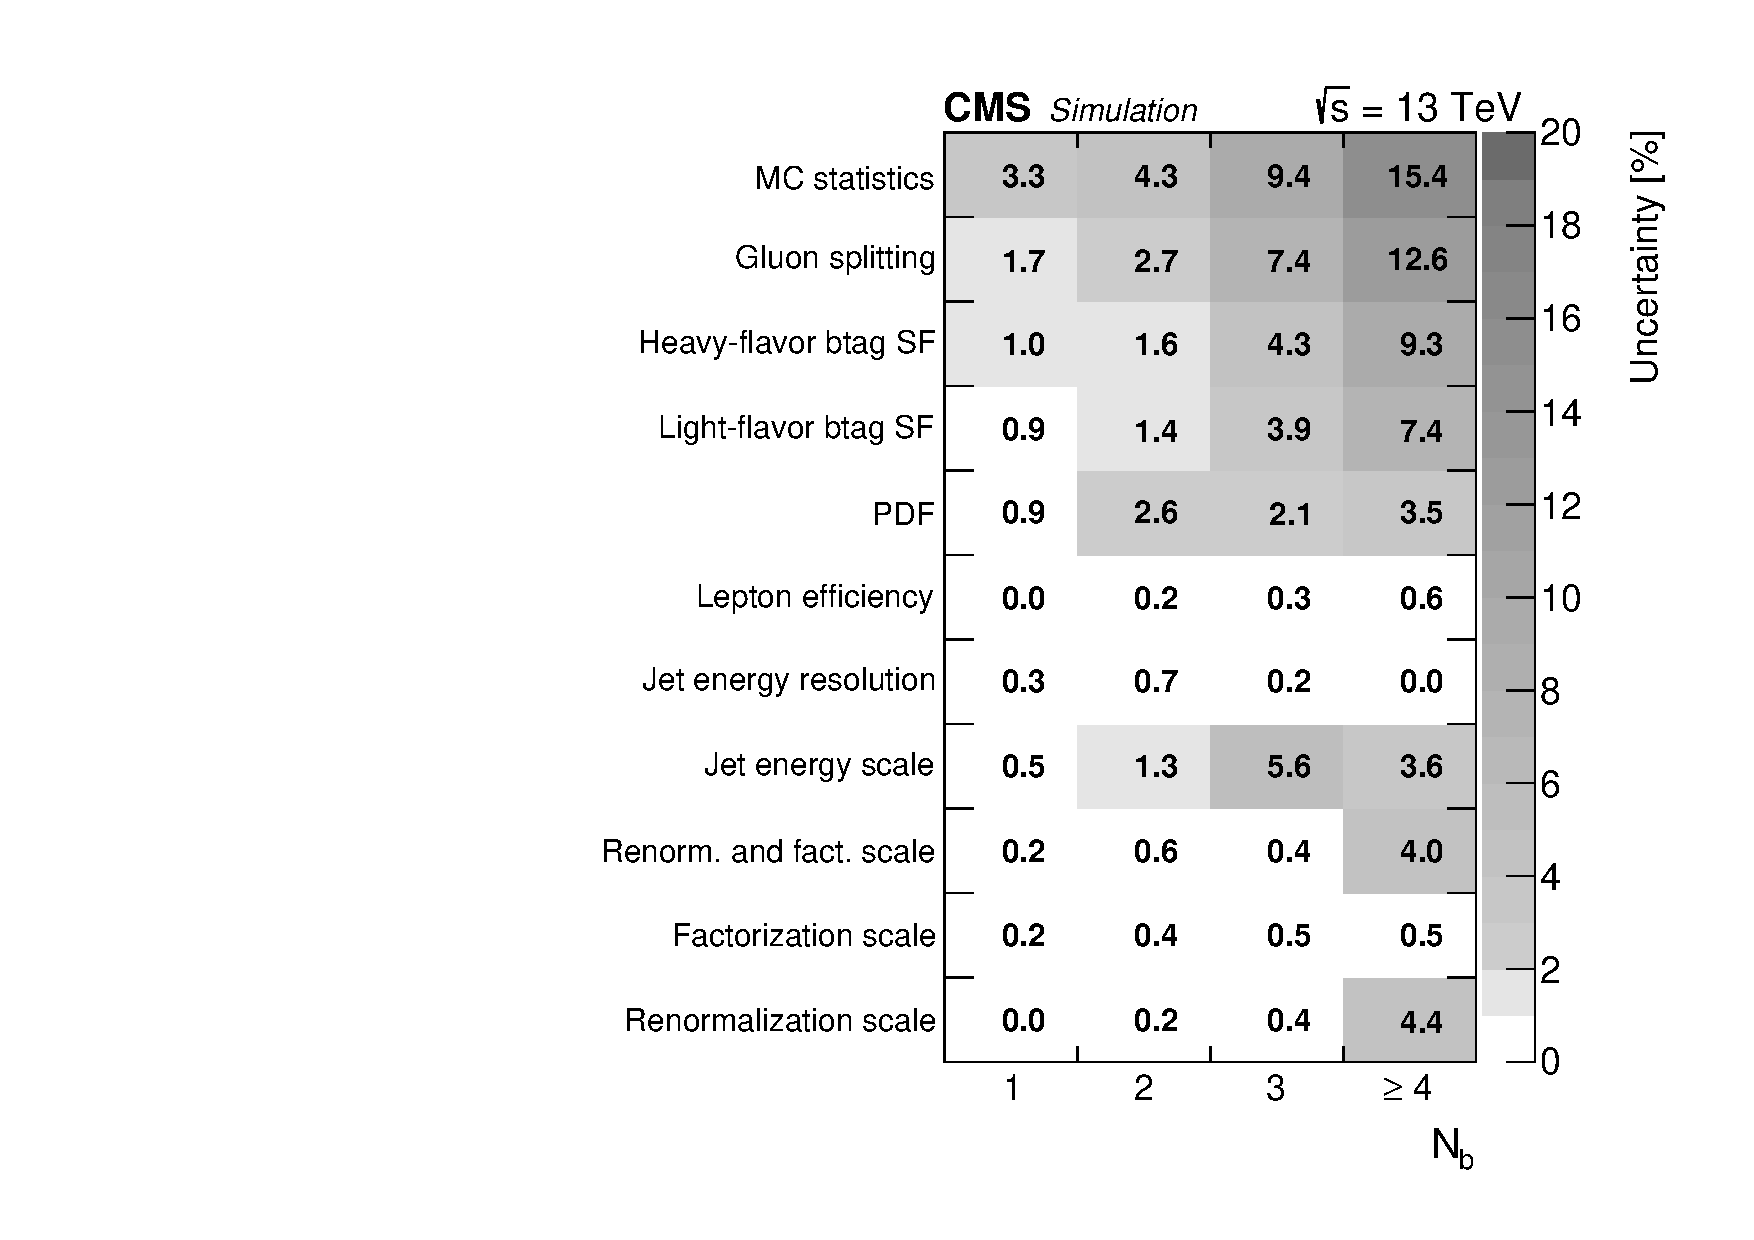
\includegraphics[angle=0,width=0.45\columnwidth]{fig/table_bkg_systs_bin20.pdf}
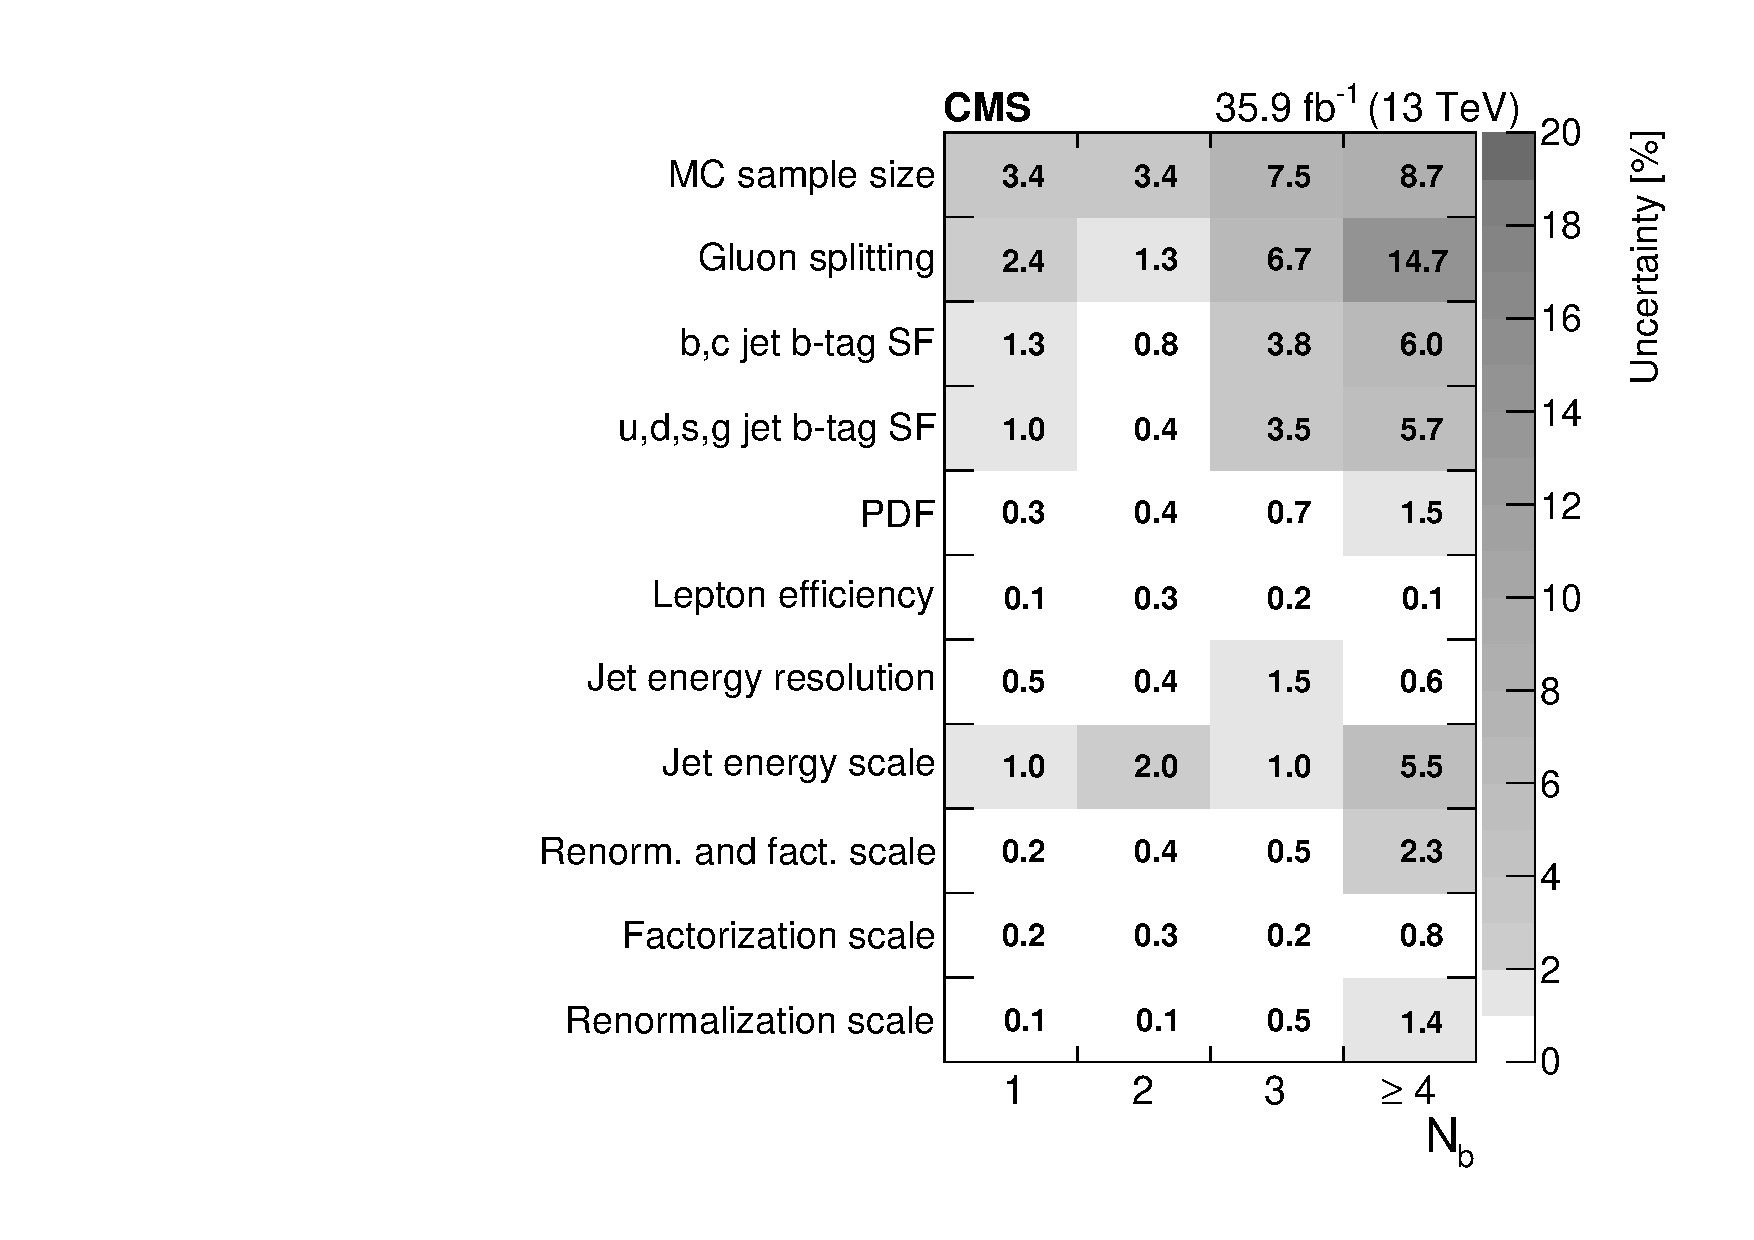
\includegraphics[angle=0,width=0.45\columnwidth]{fig/table_bkg_systs_bin21.pdf}
\end{center}
\caption{Background systematic uncertainties (in percent) for the $\Njets \geq 8$, $500 < \MJ \leq 1000~\GeV$ (left) and $\Njets \geq 8$, $\MJ > 1000~\GeV$ (right) bins.
The bottom row shows the total uncertainty for a given \Nb bin by summing in quadrature all uncertainties.
These values are similar for other bins.}
\label{fig:bkg_sys_tables}
\end{figure}

\begin{subsection}{\Nb Distribution With NLO Precision}

As the nominal \Nb distribution shape is generated at LO precision, it is important to verify that the size of NLO effects is small and covered by the experimental uncertainties.
To do this, the \Nb distributions of \ttbar samples generated at LO precision with the default \MGatNLO~2.2.2 generator and samples generated at NLO precision with \POWHEG~2.0 are compared after the baseline selection.
In order to evaluate only the shape differences between the two samples, the normalization of the \MGatNLO sample is scaled to match that of the \POWHEG sample.
The comparison of the two distributions, shown in Figure~\ref{fig:nlo_nb_comparison}, is conducted in bins of \Njets and indicates a disagreement of only about $5\%$.
This disagreement is small and subdominant to the experimental uncertainties previously discussed and no additional uncertainty is applied.

\begin{figure}[tbp!]
\begin{center}
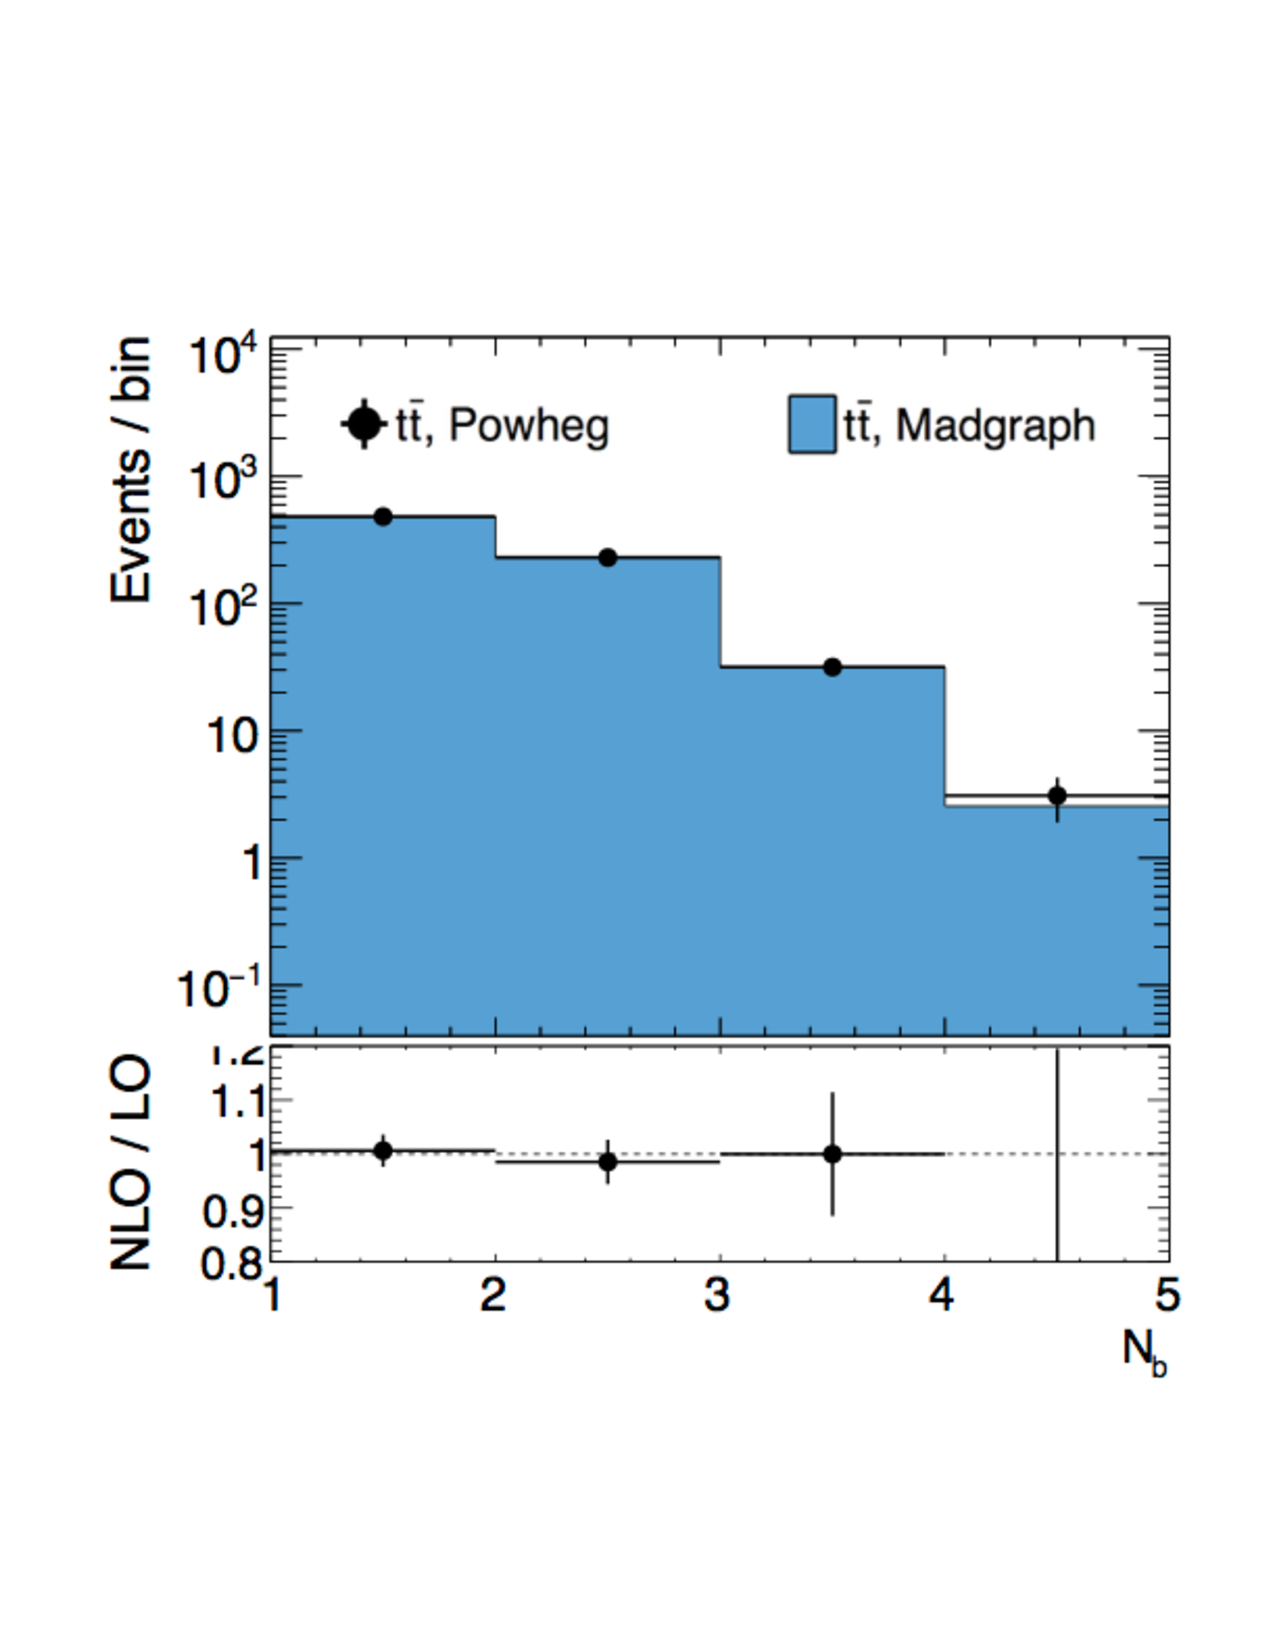
\includegraphics[angle=0,width=0.30\columnwidth]{fig/nlo_comparison_lownjet.pdf}
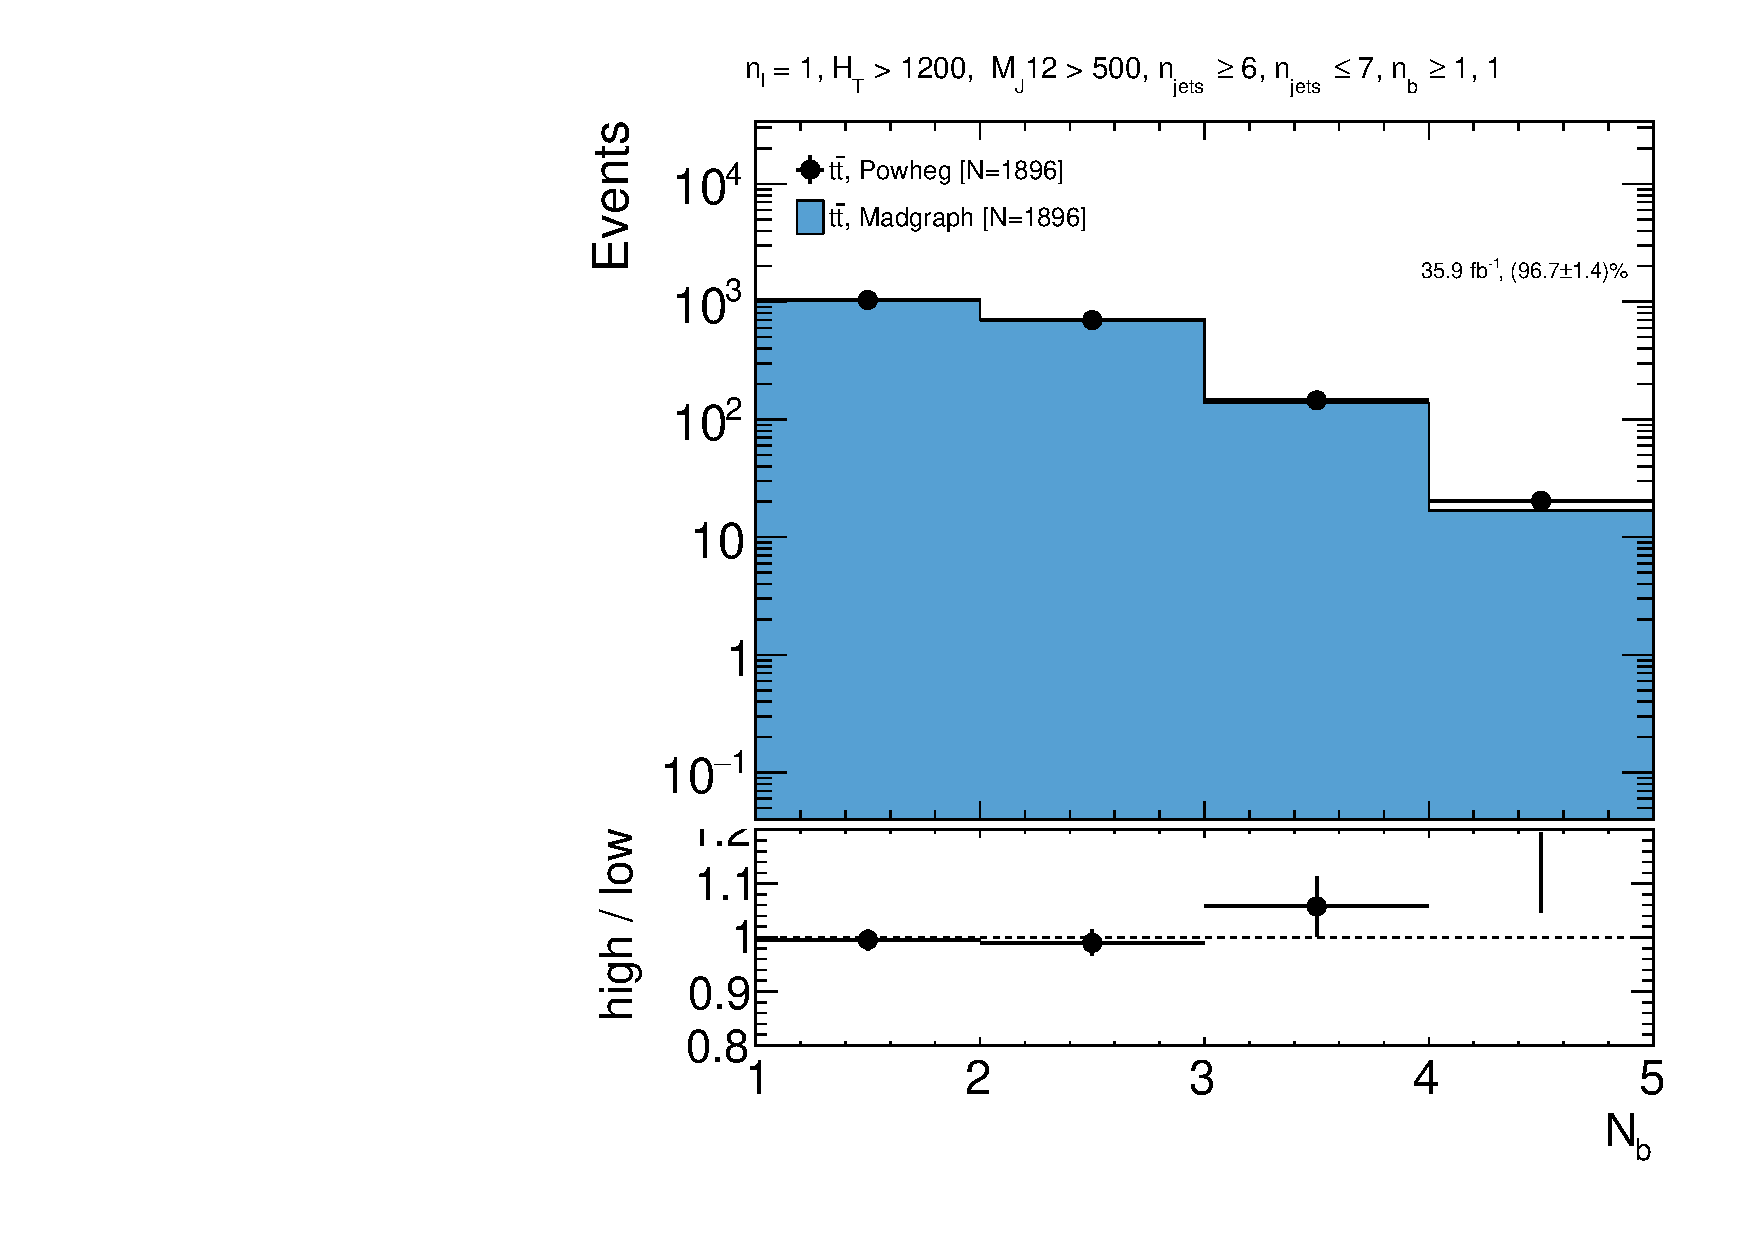
\includegraphics[angle=0,width=0.30\columnwidth]{fig/nlo_comparison_mednjet.pdf}
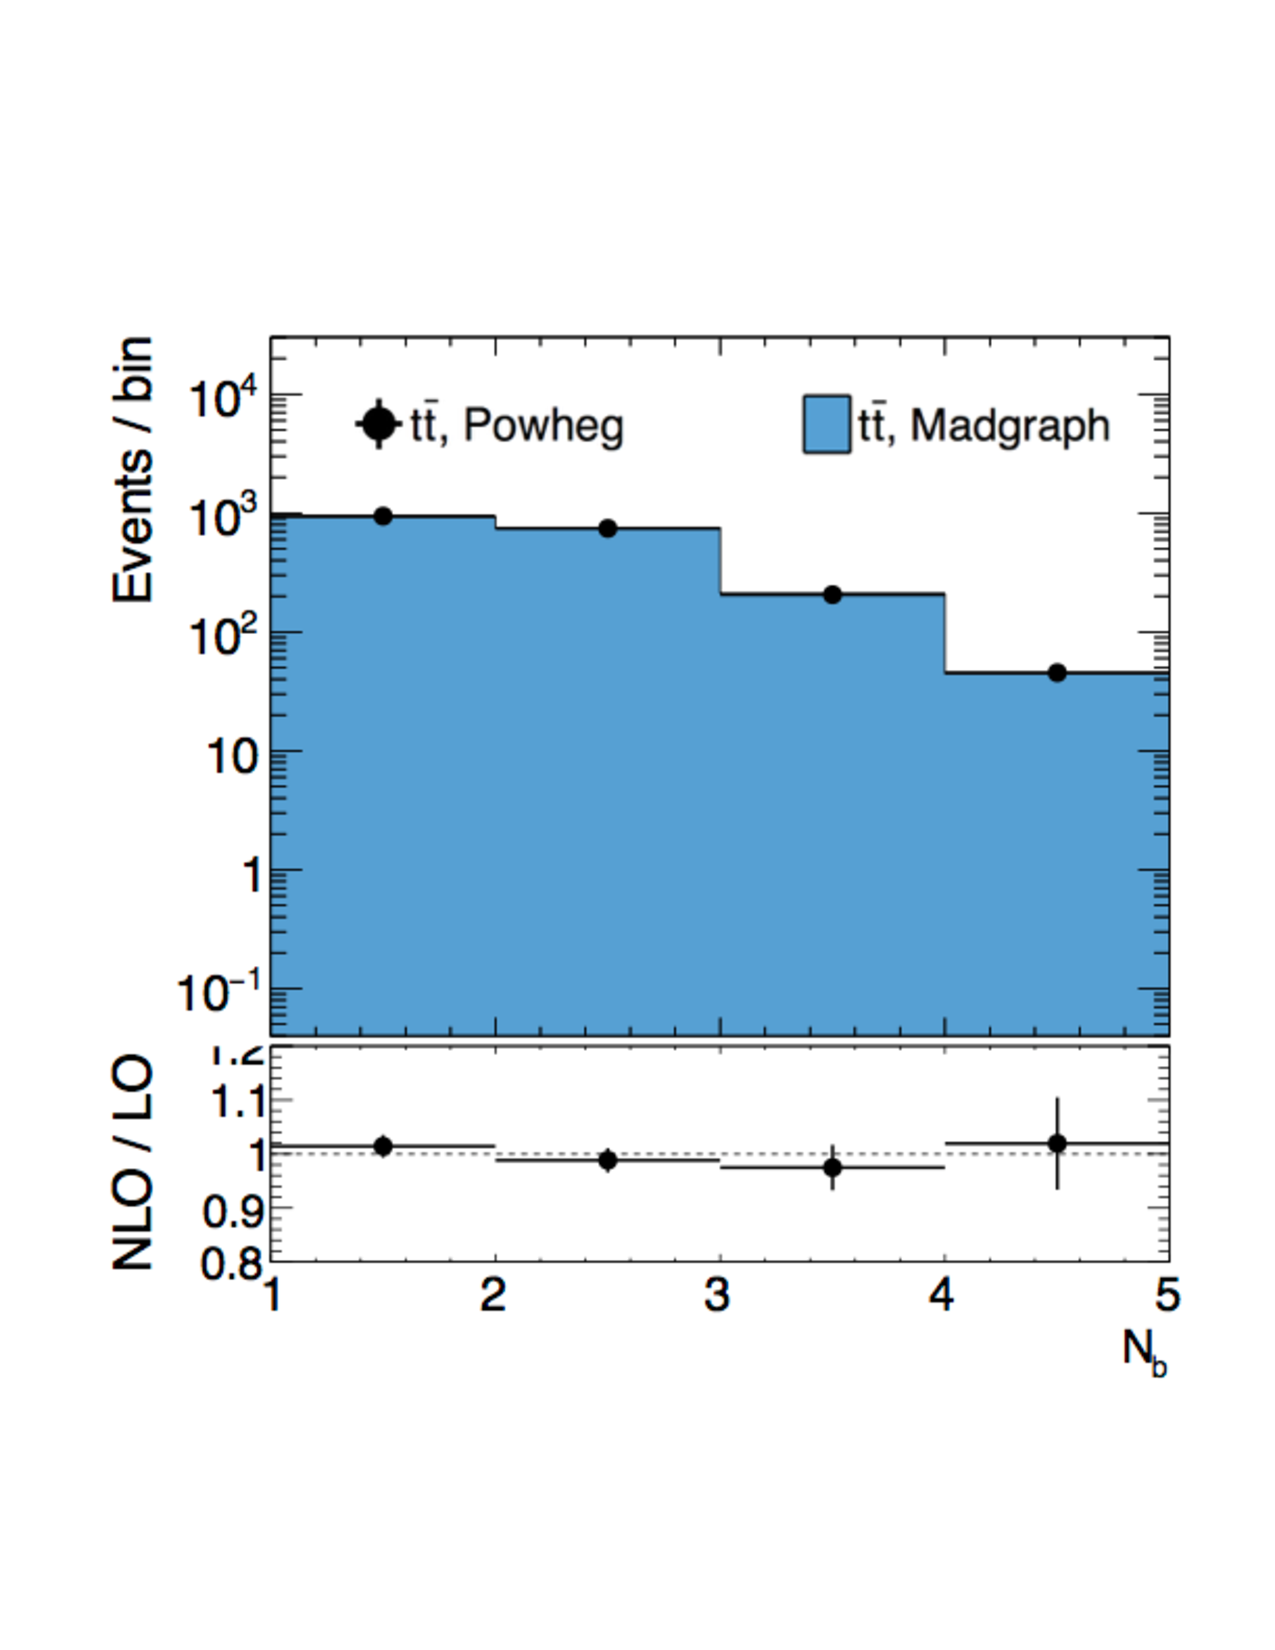
\includegraphics[angle=0,width=0.30\columnwidth]{fig/nlo_comparison_highnjet.pdf}
\end{center}
\caption{Comparison of the \Nb distribution for a sample generated at LO precision with \MGatNLO~2.2.2 (blue histogram) with that of one generated at NLO precision with \POWHEG~2.0 (data points).
The comparison is done after the baseline selection and in bins of $4 \leq \Njets \leq 5$ (left), $6 \leq \Njets \leq 7$ (middle), and $\Njets \geq 8$ (right).
In order to evaluate only shape differences, the \MGatNLO sample is normalized to match the normalization of the \POWHEG sample.}
\label{fig:nlo_nb_comparison}
\end{figure}

Given the level of agreement between the two samples, the \MGatNLO sample is used in this analysis as the sample size is significantly larger than that for the \POWHEG sample.

\end{subsection}

\end{section}

\begin{section}{Signal Systematics}

Several of the systematic uncertainties affecting the signal yield are evaluated in the same way as the background yield.
These are the uncertainties due to gluon splitting, lepton selection efficiency, jet energy scale, jet energy resolution, b~tagging scale factors, simulation sample size, integrated luminosity, and theoretical uncertainties.
All systematic variations affect both the \Nb shape and normalization, except for the gluon splitting uncertainty, which is taken to affect only the \Nb shape.

The number of jets from ISR produced in the signal simulation is reweighted based on comparisons between data and simulated \ttbar samples.
The reweighting factors vary between 0.92 and 0.51 for the number of ISR jets between 1 and $\ge6$.
One half of the deviation from unity is taken as the systematic uncertainty in these reweighting factors.

The systematic uncertainties affecting the signal \Nb shape are shown in Figure~\ref{fig:sig_sys_tables} for the most sensitive bins in a model with $m_{\glu} = 1600~\GeV$.
The dominant signal systematic uncertainties arise from the limited simulation sample size, the b~tagging efficiency scale factors, and the ISR modeling.
There is no systematic uncertainty taken for pileup reweighting, as the signal efficiency is found to be insensitive to the number of pileup interactions, which is shown in Table~\ref{tab:sig_pu_dependence}.

\begin{figure}[tbp!]
\begin{center}
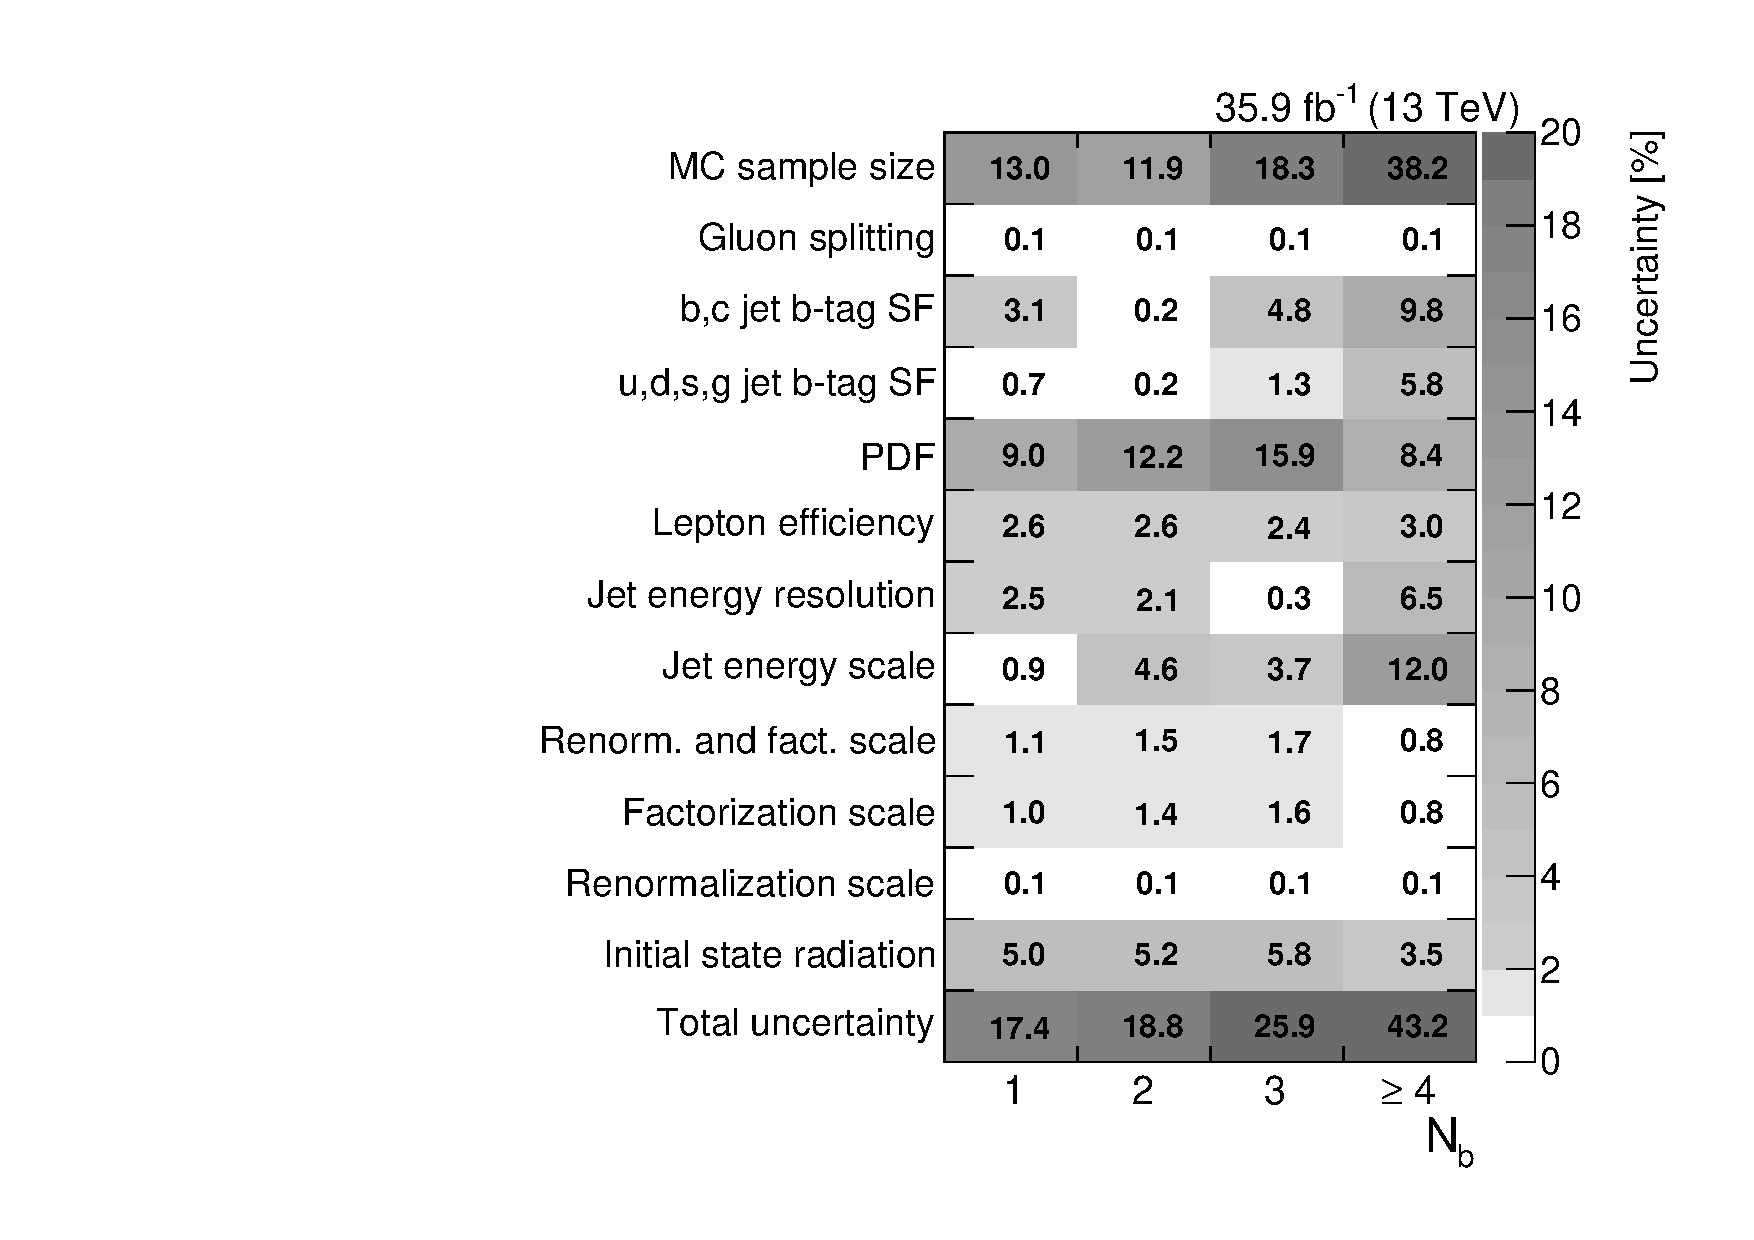
\includegraphics[angle=0,width=0.45\columnwidth]{fig/table_sig_systs_bin20_m1600.pdf}
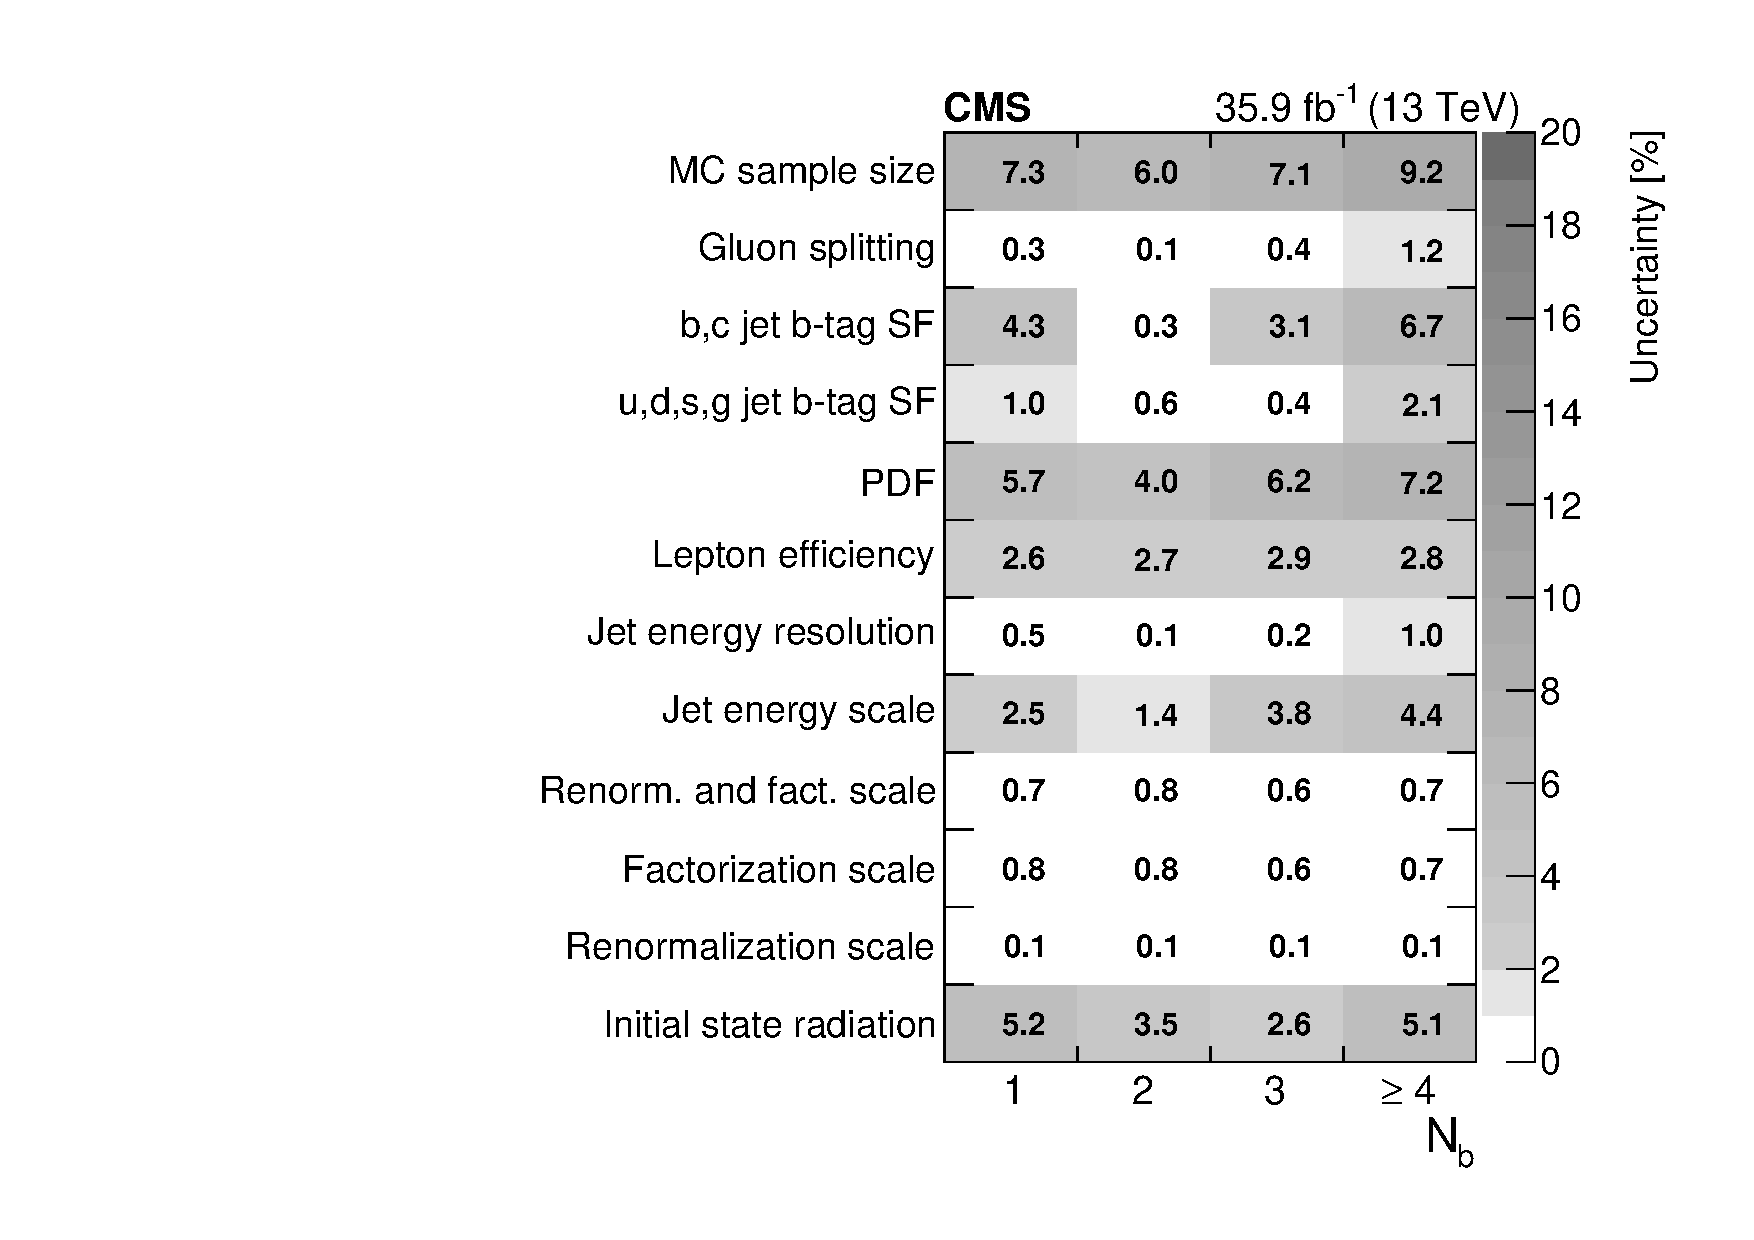
\includegraphics[angle=0,width=0.45\columnwidth]{fig/table_sig_systs_bin21_m1600.pdf}
\end{center}
\caption{Systematic uncertainties (in percent) for a $\mglu = 1600~\GeV$ signal and for the $\Njets \geq 8$, $500 < \MJ \leq 1000~\GeV$ (left) and $\Njets \geq 8$, $\MJ > 1000~\GeV$ (right) bins.
The bottom row shows the total uncertainty for a given \Nb bin by summing in quadrature all uncertainties.
These values are similar for other bins.}
\label{fig:sig_sys_tables}
\end{figure}

\begin{table}[tbp!]
\centering
\begin{tabular}{ |c|c|c| }
\hline
$N_{PV}^{true} \leq 20$ & $20 < N_{PV}^{true} \leq 40$ & $N_{PV}^{true} > 40$ \\ \hline
$8.0 \pm 0.5\%$ & $8.1 \pm 0.4\%$ & $7.5 \pm 1.5\%$ \\ \hline
\end{tabular}
\caption{The signal efficiency of the most sensitive bin $\Njets \geq 8$, $\MJ > 1000~\GeV$ for a 1600~\GeV gluino in various bins of the number of truth-level primary vertices.}
\label{tab:sig_pu_dependence}
\end{table}

\end{section}
